\documentclass[a4,12pt]{book}
\usepackage[portuguese]{babel}
\usepackage[utf8]{inputenc}
\usepackage{graphicx}
\usepackage{amsmath,amssymb,amsthm}
\usepackage{tikz}

\newtheorem{example}{Exemplo}
\newtheorem{exercicio}{Exercício}
\newtheorem{definition}{Definição}
\newtheorem{theorem}{Teorema}

\newcommand{\xor}{\oplus}

\begin{document}

\bibliographystyle{alpha}

\author{Márcio Moretto Ribeiro}

\title{Segurança da Informação}

\maketitle

\tableofcontents

\chapter*{Apresentação}

Essas são notas de aula da disciplina Segurança da Informação ministrados no segundo semestre de 2017 para as turmas do período diurno e noturno do curso de Sistemas de Informação da Escola de Artes Ciências e Humanidades (EACH) da USP.
A primeira versão desta apostila foi escrita para o curso de verão ministrado entre os os dias 2 e 6 de fevereiro de 2015 também no campus leste da Universidade de São Paulo. 
O curso de verão foi oferecido como parte das atividades do projeto de Privacidade e Vigilância do Grupo de Políticas Públicas em Acesso à Informação (GPoPAI) e foi inspirado pelo curso online oferecido gratuitamente pela plataforma Coursera e ministrado pelo professor D. Boneh.

Aos alunos que pretendem se aprofundar no tema sugerimos as seguintes referências bibliográficas:

\begin{itemize}
\item J. Katz e Y. Lindell - {\em Introduction to Modern Cryptography}
\item W. Stallings - {\em Criptografia e Segurança da Informação}
\item C. Paar e J. Pelzl - {\em Understanding Cryptography}
\end{itemize}

Agradecemos aos alunos que participaram do curso de verão em 2015 e dos cursos de gradução em 2016 e 2017, suas contribuião serviram de importante feedback para escrita dessas notas.

Alguns direitos sobre o conteúdo desta apostila são protegidos pelo autor sob licença Creative Commons
Attribution-NonCommercial-ShareAlike 4.0 International (CC BY-NC-SA 4.0). Ou seja, você  é livre para distribuir cópias e adaptar este trabalho desde que mantenha a mesma licença, dê o devido crédito ao autor e não faça uso comercial.

\begin{center}
  
\includegraphics[width=.3\textwidth]{imagens/cc.png}
\end{center}
\chapter{Introdução}

\section{Privacidade}
\label{sec:privacidade}

As primeiras tentativas de conceitualizar a privacidade datam do final do século XIX.
Em um famoso artigo de 1890, os colegas da faculdade de direito de Bosto, Louis Brandeis e Samuel Warren denunciam que o advento da fotografia instantânea e o jornalismo haviam ``invadido o recinto sagrado da vida privada'' ferindo o que eles apontam como o direito individual de ``ser deixado em paz''.
Assim, eles argumentam que o escopo do direito comun ({\em Common Law}), que originalmente se concentrava apenas na proteção contra agreções e já havia sido ampliado para incluir a proteção à propriedade deveria ser novamente alargado para finalmente reconhecer a ``natureza espiritual do homem'' \cite{Warren1890}.

Essa visão da privacidade como proteção à intimidade ou, nas palavras dos autores, como o ``direito de ser deixado em paz'' é a chave de interpretação que prevalece no debate público.
Duas contribuições que não fogem a esse espírito, porém, merecem destaque nessas notas introdutórias.
Em um influente artigo de 1977, Richard Posner propõe que as disputas sobre direito à privacidade sejam interpretadas em sua dimensão econômica.
Para Posner, as informações privadas possuem valor. 
De um lado há o interesse de quem busca construir uma imagem pública sobre si, uma reputação e, de outro, há o interesse de se conhecer o outro para melhor saber como se relacionar com ele ou aprender sobre sua trajetória.
Caso fosse permitido qualquer tipo de intrusão à privacidade, o efeito seria um esforço maior em não revelar, ou inclusive não produzir, dados potencialmente valiosos.
Assim, a questão da privacidade, se resumiria a uma questão de eficiência econômica.
Caberia ao legislador regular o direito ao controle da reputação procurando um equilíbrio que maximizasse os fluxos de informação \cite{Posner77}. 

O risco tanto para o indivíduo cuja paz é  perturbada pelas fotos não autorizadas, quanto para aquele que perde o controle sobre sua reputação é de que algo que pertencia a sua esfera privada se tornasse pública.
Para Nissenbaum, essa dicotomização entre público e privado não dá conta dos problemas associados a quebra de privacidade.
Por exemplo, um paciente espera que as informações sobre sua condição de saúde sejam eventualmente compartilhadas com outros médicos ou médicas com o intuito de melhor diagnosticá-lo, assim como um cliente espera que seu gerente de banco use suas informações bancárias para sugerir-lhe melhores investimentos.
Porém, há uma flagrante quebra de privacidade se as informações médicas forem compartilhadas com o banco, com quem eventualmente o paciente negociará um plano de saúde.
Esse cenário exemplifica o que a autora chama de rompimento da ``integridade contextual do fluxo de informações'' \cite{Nissenbaum09}.

\section{Vigilância}
\label{sec:vigilancia}
% Foucalt e Deleuze

Associado ao tema da privacidade, mas ligado a outra matriz teórica, estão os debates sobre vigilância.
Diferente dos estudos sobre privacidade cujos principais autores são juristas preocupados com o direito individual, os esttudos sobre vigilância focam em relações de poder.
Foucault descreve a vigilância como uma técnica que teria alterado profundamente as formas de exercer o poder durante os séculos XVII e XIX.
O poder do senhor feudal durante a idade média era exercído por meio do suplício, a pena corporal em que o açoitado pedia misericórdia eventualmente concedida.
Após a revolução francesa o suplício foi sendo substituido pela prisão e aos poucos seria desenvolvida a técnica da disciplina e da vigilância.
Para o autor, a imagem que melhor descreve a técnica é uma estrutura arquitetônica proposta por Jeremy Bentham no final do século XVII.
Bentham arquitetou um modelo de prisão em que os vigias ficariam no centro aonde poderiam observar todas as celas, porém, aqueles que ocupam as celas não poderiam observar o vigia.
A sensação constante de estar sendo vigiado introgetaria a disciplina, outra técnica deste período, nos condenados.
O propósito da vigilância e da disciplina é o de produzir corpos dóceis e obedientes \cite{Foucault96}.

Em 1992, em um curto texto, Giles Deleuze propos uma atualização dos conceitos de Foucault que antecipariam o que hoje compreendemos como vigilância.
Na sociedade disciplinar, descrita por Foucault, durante a vida o indivíduos passa de uma instituição disciplinar a outra: da escola, ao exército, do exército à fábrica e da fábrica ao hospital.
Cada instituição disciplina o indivíduo e o modela da maneira mais eficiente à instituição.
Na sociedade do controle, conforme descrita por Deleuze, o poder é exercido de maneira mais intermitente e mais sutil.
O indivíduo prototípico da sociedade do controle seria o endividado cujo controle atravessa as instituições \cite{Deleuze92}.

\section{Marco Regulatório}
\label{sec:marco-regulatorio}
% Mayer-Schonberger

Antes ainda dos primeiros computadores, as chamadas máquinas Hollerith revolucioram a capacidade de processamento de dados.
Durante a década de trinta elas dinamizaram o processamento dos dados do censo nos EUA e na década de 40 foram usadas pelos nazistas para classificar aqueles, principalmente judeus, mas também comunistas e homossexuais, que deveriam ser transportados para os guetos, dos guetos para os campos de concentração e finalmente para as câmaras de gás \cite{Black01}.
Finda a guerra, a evolução dos modernos Estados de bem estar social Europeu e seu necessário processamento massivo de dados casou muito bem com o desenvolvimento computacional e assustou os cidadãos com sua centralidade de processamento.
Assim, começaram a surgir as primeiras leis de proteção de dados pessoais.

Mayer-Schonberger argumenta que, uma vez que as leis de proteção de dados pessoais na Europa partem todas das mesmas bases e diferem apenas em detalhes, é mais frutífero estudá-las em conjunto do que seguindo uma análise comparativa.
Ele propõe uma abordagem geracional como se existisse uma tendência evolutiva das normas.
A primeira geração, no começo dos anos 70, focou na regulamentação técnica dessas bases centralizadas de dados.
O surgimento de mini-computadores, que favorecia o processamento descentralizado, levou a uma adaptação na legislação.
A segunda geração, no final dos anos 70, focou na liberdade negativa, o direito civíl de "ser deixado em paz" nas palavras de Brandeis e Warren.
A autonomia do indivíduo é, porém, contraposta a sua inclusão nos programas sociais do Estado.
Então, a terceira geração legislativa, em meados dos anos 80, foge um pouco das liberdades negativas e foca em uma abordagem participativa de autodeterminação informacional.
A pergunta deixa de ser se alguém quer participar ou não de processos sociais, mas como.
Ainda assim, porém, os indivíduos estavam em uma posição frágil nas relações de negociação o que os levava, via de regra, a abdicar dos seus direitos.
A quarta geração, de meados dos ano 90, procurou de um lado equalizar as posições de negociação ainda apostando na autonomia do indivíduo, mas também incluiu diversos mecanismos mais paternalistas excluindo certas liberdades participativas e as sujeitando à proteção juridica obrigatória.
Nessa fase surgem órgãos de defesa, não apenas de auxílio aos cidadãos, mas com papel decisório para delibera contra violações \cite{Mayer-Schonberger97}.

No Brasil, o Marco Civil da Internet aprovado em 2013 não aborda diretamente as questões de proteção de dados pessoais.
Carecemos de um marco legal que imponha, pelo menos, que o uso de dados pessoas dependa necessariamente do consentimento explicito e informado e cuja autorização seja dada para um fim específico.

\section{Vigilância Digital em Massa}
\label{sec:vigil-digital}

Em 2013 Edward Snowden revelou ao mundo o alacance dos programas de vigilância em massas das agências de espionagem dos EUA.
O jornalista Glen Greenwald e a cineasta Laura Poitras divulgaram o caso em uma serie de matérias e um documentário \cite{Greenwald14, Poitras14}.
O vazamento demonstra que a agência de segurança nacional dos EUA (NSA) tem acesso a toda a comunicação por telefone e pelos principais meios de comunicação online do mundo.
O moderno modelo de negócios das empresas de internet baseado na propaganda direcionada depende da construção de perfis digitais que por sua vez dependem da produção e aquisição de uma grande escala dados pessoas.
Essa competição por dados pessoais cria o que chamamos de pontos únicos de falha.
A violação dessas bases permitiu à NSA produzir um banco de dados pesquisável da agência possui toda comunicação pública e privada que passa pelos servidores da Google, do Facebook, da Microsof e da Apple.

A vigilância digital em massa eleva o problema da privacidade para um outro patamar.
Não se trata apenas de proteger a intimidade, ou a inviolabilidade do lar, ou do controle na construção da reputação. 
Nesse contexto, o problema da privacidade é também coletivo.
A privacidade deve ser também enchergada como um direito civil, uma limitação ao poder do estado de antecipar as ações de grupos políticos. 
Para tanto, é preciso de ação politica de concientização, de regulamentação para restringir o poder das empresas que controlam o armazenamento dos dados pessoais e também desnvolvimento técnico. 

\section{Segurança da Informação}
\label{sec:seg-inf}

A internet é um meio intrinsecamente promíscuo \cite{}.
Por uma decisão de projeto, não temos controle por onde nossas informações passam quando nos comunicamos pela rede.
Conforme produzimos mais informações pessoais e permitimos que elas circulem, maior o risco de quebra da integridade dos fluxos contextuais.
Em particular há atores poderosos com capacidade conhecida de observar a comunicação em escala global o que traz um risco coletivo tanto à soberania nacional dos países perifércos, como o Brasil, quanto à democracia.
A regulamentação, absolutamente necessaria para controlar minimamente esses processos e garantir pelo menos o consentimento no uso de nossas informações pessoais, certamente não é suficiente.
A compreensão, o desenvolvimento e a difusão de ferramentas de segurança da informação podem colaborar nesse sentido.
Concluiremos o capítulo com uma história motivadora.

Após as denúncias de Snowden houve uma espécie de consenso nos meios ativistas sobre a importância de focar forças em desenvolver ferramentas que garantissem a criptografia ponta a ponta.
O paradigma mais comum de comunicação na rede é criptografar a comunicação entre cada cliente e o servidor.
Como já dissemos, conforme poucos servidores consentram a maior parte da comunicaçõ online, a informação armazenada nesses servidores passa a ser um bem muito requisitado.
A ideia para superar isso seria criptografar a comunicação entre clientes.
Assim, a informação armazenada nos servidores não seria compreensível seja pelos engenheiros das empresa que controla a comunicação, seja para um ator externo como um hacker ou a NSA.
O principal protocolo de criptografia ponta a ponta na época era o PGP, que havia sido criado no começo da década de 90, antes do advento da web.
As tentativas mal sucedidas de ressucitar o protocolo logo foram substituídas por um esforço em atualizá-lo.
Duas aplicações que garantiam criptografia ponta a ponta em celulares se popularizaram nesse período: Telegram e o Textsecure.
A primeira foi desenvolvida por uma compania russa e oferece serviço de criptografia ponta a ponta em comunicação síncrona usando um protocolo desenvolvido por seus engenheiros.
A segunda foi desenvolvida por uma pequena empresa no Vale do Silício e se inspirou no protocolo OTR, que por sua vez se inspirou no PGP, adaptando-o para o contexto assíncrono mais adequado para a comunicação móvel.
Os esforços de ativistas em promover esse tipo de ferramenta culminou com a adoção do protocolo do Textsecure, rebatizado como Signal, no Whatsapp, a ferramenta de comunicação móvel mais usada no mundo todo.
A popularização da criptografia ponta a ponta em grande parte da comunicação interpessoal muda muito o cenário de proteção de direitos civis e de liberdade de organização.
É certo que os metadados das comunicações - quem fala com quem, quando e de onde - não estão protegidos, é certo que a maior parte da comunicação interpessoal não está livre de intrusão seja de hackers, seja de agências governamentais, é certo que há serviços - como agenda online - em que simplesmente não há alternativa segura e, portanto, é necessaria muita ação política e desenvolvimento técnico nessa área.
\chapter{Cifras Clássicas}
\label{cha:cifras-classicas}

Como argumntamos no primeiro capítulo, a internet é um meio de comunicação promíscuo.
As partes que se comunicam pela rede não tem controle sobre por quais caminhos sua comunicação irá trafegar.
Essa característica, porém, não se restringe a esse meio.
Durante o século XVIII, por exemplo, toda correspondência que passava pelo serviço de correios de Viena na Austria era encaminhada para um escritório -- {\em black chamber} -- que derretia o selo, copiava seu conteúdo, recolocava o selo e reincaminhava para o destinatário.
Todo esse processo durava cerca de três horas para não atrasar a entrega.
Como a Áustria, todas as potências européias desse período operavam suas {\em back-chambers}.
As invenções do telegrafo e do rádio só facilitaram a capacidade de criar grampos, no primeiro caso, ou simplesmente captar a comunicação no segundo \cite{Kahn96}.

Partiremos, portanto, do seguinte modelo de comunicação.
Duas partes, o remetente e o destinatário, buscam se comunicar.
Tradicionalmente denominaremos o remetente de Alice e o destinatário de Bob.
Nossa suposição principal é que o canal de comunicação entre as partes é inseguro.
Ou seja, assumiremos que terceiros, que denominaremos de Eva, são capazes de observar as mensagens que trafegam pelo canal de comunicação.
Essa suposição é conhecida em alguns meios como ``hipótese da comunicação hacker''.
Para efeitos deste curso, sempre assumiremos essa hipótese.

A {\em criptografia} (do grego ``escrita secreta'') é a pratica e o estudo de técnicas de comunicação segura na presença de terceiros chamados de {\em adversários}.
A {\em criptoanálise}, por sua vez, é o estudo e a análise dos sistemas de informação com a intenção de desvelar seus segredos.
Nosso primeiro desafio no curso é apresentar sistemas de comunicação que garantam a {\em confidencialidade}.
Ou seja, toda mensagem enviada de Alice para Bob deve ser compreensível apenas para Alice e Bob e deve ser incompreensível para Eva:
\begin{center}
\begin{tikzpicture}[node distance=2cm,auto,>=latex]
\node (alice) {Alice};
\node (bob) at (10,0) {Bob};
\node (eva) at (5,2) {Eva};
\draw[->] (alice) -> node[above]{mensagem} (bob);
\path[->] (eva) edge (5,.5);
\end{tikzpicture}
\end{center}

Se a importância da comunicação confidencial entre civis tem se tornado cada vez mais urgente, no meio militar é difícil remontar suas origens. 
Suetônio (69 - 141) por volta de dois mil anos atrás descreveu como o imperador Júlio César (100 a.c. - 44 a.c.) escrevia mensagens confidenciais:


\begin{quote}
  ``Se ele tinha qualquer coisa confidencial a dizer, ele escrevia cifrado, isto é, mudando a ordem das letras do alfabeto, para que nenhuma palavra pudesse ser compreendida. 
  Se alguém deseja decifrar a mensagem e entender seu significado, deve substituir a quarta letra do alfabeto, a saber 'D', por 'A', e assim por diante com as outras.''
\end{quote}

O esquema que chamaremos de cifra de César é ilustrado pelo seguinte exemplo:

\begin{verbatim}
Mensagem: transparenciapublicaopacidadeprivada
Cifra:    XUDQVSDUHQFLDSXEOLFDRSDFLGDGHSULYDGD
\end{verbatim}

Como descrito Suetônio, a regra para encriptar uma mensagem consiste em substituir cada letra da mensagem por aquela que está três posições a sua frente na ordem alfabética.
Para descriptografar a cifra, substituir cada letra por aquela que está três posições atrás.
O problema com este tipo de sistema é que basta conhecer a regra de criptografia para decifrá-lo.
Em outras palavras, o segredo da cifra é sua própria regra.
 
Embora técnicas de criptografia e criptoanálise existam desde o império romano, foi com o advento do teléfgrafo e sua capacidade de comunicação eficiente, que o campo se estruturou.
No fim do século XIX Auguste Kerckhoff estabeleceu seis princípios que as cifras militares deveriam satisfazer:
\begin{enumerate}
\item O sistema deve ser indecifrável, se não matematicamente, pelo menos na prática.
\item O aparato não deve requerer sigilo e não deve ser um problema se ele cair nas mãos dos inimigos.
\item Deve ser possível memorizar uma chave sem ter que anotá-la e deve ser possível modificá-la se necessário.
\item Deve ser possível aplicar a sistemas telegráficos.
\item O aparato deve ser portátil e não deve necessitar de muitas pessoas para manipulá-lo e operá-lo.
\item Por fim, dadas ascircunstâcias em que ele será usado, o sistema deve ser fácil de usar e não deve ser estressante usá-lo e não deve exigir que o usuário conheça e siga uma longa lista de regras.
\end{enumerate}

O segundo princípio ficou conhecido como {\em princípio de Kerckhoff}.
Ele estabelece que a regra usada para criptografar uma mensagem, mesmo que essa regra esteja codificada em um mecanismo, não deve ser um segredo e não deve ser um problema caso ela caia nas mãos do adversário.
Nas palavras de Claude Shannon: ``o inimigo conhece o sistema''.
Whitfield Diffie coloca o debate nos seguintes termos:

\begin{quote}
``Um segredo que não pode ser rapidamente modificado deve ser interpretado como uma vulnerabilidade''
\end{quote}

Ou seja, em uma comunicação confidencial as partes devem compartilhar algo que deve ser ``possível de modificar caso necessário''.
Esse segredo compartilhado é o que chamaremos de {\em chave} da comunicação e assumiremos que ela é a única parte sigilosa do sistema.
Trazendo o debate para uma discução mais moderna, o sigilo do código-fonte de um sistema não deve em hipótese alguma ser aquilo que garanta sua segurança.

O modelo de {\em criptografia simétrica}, portanto, pode ser descrito da seguite maneira:
o remetente usa um algoritmo público ($E$) que, dada uma chave ($k$), transforma uma mensagem ($m$) em um texto incompreensível chamado de {\em cifra} ($c$), a cifra é enviada para o destinatário por um meio assumidamente inseguro (hipótese da comunicação hacker) e o destinatário utiliza a mesma chave em um algoritmo ($D$) que recupera a mensagem a partir da cifra.

\begin{center}
\begin{tikzpicture}[node distance=2cm,auto,>=latex]
\node (alice) at (0, 2){Alice};
\node (bob) at (10, 2) {Bob};
\node (eva) at (5, 2) {Eva};

\node (m1) at (0,1) {$m$};
\node (k1) at (0,-1) {$k$};
\node (E)  at (2,0) {$E(k,m) = c$};
\node (D)  at (8,0) {$D(k,c) = m$};
\node (k2) at (10,-1) {$k$};
\node (m2) at (10,1) {$m$};

\path[->] (eva) edge (5,1);
\draw[->] (m1) -> (E);
\draw[->] (k1) -> (E);
\draw[->] (D) -> (m2);
\draw[->] (k2) -> (D);
\draw[->] (E) -> node[above]{$c$} (D);
\end{tikzpicture}
\end{center}

\section{Cifra de Deslocamento}
\label{sec:cifra-deslocamento}

O que chamamos na seção anterior como ``cifra de César'' não deve ser propriamente considerado uma cifra, pois não possui uma chave.
Porém, é possível e simples adaptar esse esquema para incorporar uma chave.
Para tanto faremos a seguinte alteração no esquema.
Ao invés de deslocar as letras sempre três casas para frente vamos assumir que foi sorteado previamente um número $k$ entre $0$ e $23$.
Esse número será a chave da comunicação e, portanto, assumiremos que as partes a compartilham.
O mecanismo para criptografar uma mensagem será o de deslocar cada letra $k$ posições para a direita e para descriptografá-la basta deslocar cada letra as mesmas $k$ posições para a esquerda.

Para formalizar este mecanismo vamos assumir que cada letra do alfabeto seja representada por um número: a letra {\tt a} será representada pelo $0$, a letra {\tt b} pelo $1$ e assim por diante.
O universo de todas as chaves possíveis é o conjunto $K = \{0 ... 23\}$ (chamaremos este conjunto de $\mathbb{Z}_{26}$ ou de maneira mais genérica $\mathbb{Z}_n = \{0, 1, \dots, n - 1\}$) e o universo de todas as mensagens possíveis é representado pelo conjunto $M = {\mathbb{Z}_{26}}^\star$, ou seja, todas as sequências de números entre $0$ e $23$.
Além disso, o conjunto das possíveis cifras é $C = M$.
Precisamos descrever três algorítmos:
\begin{itemize}
\item $Gen$ que gera a chave $k \in K$,
\item $E$ que recebe uma chave $k \in K$ e uma mensagem $m \in M$ e produz uma cifra $c \in C$ (i.e.: $E: K \times M \to C$) e
\item $D$ que recebe uma chave $k \in K$ e uma cifra $c \in C$ e produz uma mensagem $m \in M$ (i.e.; $D: K \times C \to M$).
\end{itemize}

Um sistema de criptografia simétrica $\Pi$ é formado por essa tripla de algoritmos $\Pi = \langle Gen, E, D \rangle$.
Além disso, precisamos garantir que quem possui a chave seja capaz de descriptografar a cifra.
Ou seja, precisamos garantir que:
\begin{displaymath}
  D(k, E(k, m)) = m
\end{displaymath}

O mecanismo que gera uma chave na cifra de substituição é bastante simples, ele simplesmente sorteia com uma distribuição de probabilidade uniforme um número entre $0$ e $23$.
Escreveremos da seguinte forma:
\begin{displaymath}
Gen := k \leftarrow \mathbb{Z}_{26}  
\end{displaymath}

Utilizaremos a partir daqui a convenção de usar uma seta da direita para esquerda indicando que será escolhido um elemento do conjunto com probabilidade uniforme.

O algoritmo para criptografar uma mensagem traz um pequeno problema.
Escreveremos $m = m_0 m_1 m_2 \dots m_n$ uma mensagem $m$ com $n + 1$ letras cuja primeira letra é $m_0$, a segunda é $m_1$ e assim por diante.
Nossa primeira tentativa de formalizar $E$ seria somar $k$ a cada uma das letras $m_i$.
O problema é que esta soma pode resultar em um valor que não corresponde a nenhuma letra i.e. $m_i + k > 23$.
Para evitar este problema utilizaremos não a aritmética convencional, mas a {\em aritmética modular}.

Dizemos que um número $a$ divide $b$ (escrevemos $a|b$) se existe um número inteiro $n$ tal que $a.n = b$.
Dois números são equivalentes módulo $n$ (escrevemos $a \equiv b\ (mod\ n)$) se $n|(b-a)$.
Em outras palavras, dois números são equivalentes módulo $n$ se o resto da divisão de cada um por $n$ for o mesmo reultado.
O conjunto de todos os números equivalentes módulo $n$ forma uma classe de equivalência que representaremos como $[a\ mod\ n] = \{b \in \mathbb{Z} : a \equiv (b\ mod\ n)\}$.
Por exemplo $[5 + 7\ mod\ 10] = [2\ mod\ 10]$ pois $5 + 7 = 12$ e o resto de $12$ por $10$ é $2$.

Estamos finalmente em condições de formalizar o sistema da cifra de deslocamento $\Pi = \langle Gen, E, D\rangle$:
\begin{itemize}
\item $Gen := k \leftarrow \mathbb{Z}_{26}$
\item $E(k, m) = [m_0 + k\ mod\ 26] \dots [m_n + k\ mod\ 26]$
\item $D(k, c) = [c_0 - k\ mod\ 26] \dots [c_n - k\ mod\ 26]$ 
\end{itemize}


\begin{example}
  Considere a palavra {\tt XUXA}.
  Usando a cifra de César com chave $k = 3$ obtemos a cifra {\tt BZBD}.

  \begin{itemize}
  \item $E(3, \textrm{\tt 24 21 24 0}) = [1\ mod\ 26] [21\ mod\ 26] [1\ mod\ 26] [3\ mod\ 26]$  
  \item $D(3, \textrm{\tt 1 21 1 3}) = [24\ mod\ 26] [21\ mod\ 26] [24\ mod\ 26] [0\ mod\ 26]$
  \end{itemize}

  Note que $[27\ mod\ 26] = [1\ mod\ 26]$ e que $[-2\ mod\ 26] = [24\ mod\ 26]$.
\end{example}



\section{Cifra de Substituição}
\label{sec:cifra-monoalfabetica}

Em 1567 a residência da rainha da Mary da Escócia foi destruída por uma explosão que levou a morte do então rei, primo de Mary.
O principal suspeito do assinato foi dispensado da pena e se casou com Mary no mês seguinte.
O episódio levou-a a prisão na Inglaterra.
Neste tempo, para a maioria dos católicos, Mary era a legítima herdeira do trono inglês - ocupado pela protestante Elizabeth I.
Durante o tempo na prisão Mary consiporou com aliados pela morte de Elizabeth.
Em 1587 Mary foi executada pelo que ficou conhecido como a conspiração de Babington.
A principal prova utilizada para a condenação foi uma troca de cartas cifradas interceptadas e decifradas \cite{Singh04}.

A cifra usada pelos conspiradores é conhecida hoje como {\em cifra de substituição} ou {\em cifra monoalfabética}.
Neste tipo de criptografia, cada letra ou par de letras é substituída por um símbolo, que pode ser inclusive uma outra letra.
Assim, a chave desse tipo de cifra é um alfabeto.


\begin{example}
  Considere a seguinte chave de uma cifra monoalfabética.
  Neste caso os símbolos utilizados letras do mesmo alfabeto em ordem embaralhada:
  \begin{verbatim}
    Alfabeto:   abcdefghijklmnopqrstuvwxyz
    Permutação: ZEBRASCDFGHIJKLMNOPQTUVWXY
  \end{verbatim}

  A partir desta chave podemos produzir textos substituindo cada letra pela letra correspondente na chave.
  Para descriptografar, basta fazer o processo inverso, a saber, substituir a letra da cifra pela do alfabeto.
  
  \begin{verbatim}
    Mensagem: transparenciapublicaopacidadeprivada
    Cifra:    QOZKPMZOAKBFZMTEIFBZLMZBFRZRAMOFUZRZ
  \end{verbatim}
\end{example}

O desfecho da história da conspiração de Babington sugere que a cifra monoalfabética não é muito segura.
De fato, no próximo capítulo discutiremos melhor as técnicas de criptonálise para este tipo de cifra.
Não obstante, até o desenvolvimento das primeiras máquinas de criptografar, versões das cifras monoalfabéticas foram eram as cifras mais populares no mundo todo.
Nos anos 70 a editora abril publicou no Brasil o famoso Manual do Escoteiro Mirim da Disney que apresentava uma cifra monoalfabética.
Mais recentemente, o curioso caso do desaparecimento de um rapaz no Acre viralizou quando seus familiares revelaram que no seu quarto havia uma coleção de livros que ele havia escrito de maneira criptografada.
Mais tarde foi descoberto que o rapaz usara uma cifra de substituição cuja chave foi eventualmente encontrada.

Para fechar esta seção buscaremos formalizar o sistema de cifra de substituição simples.
Uma {\em permutação} sobre um conjunto $\Sigma$ qualquer é uma {\em função bijetora} $p: \Sigma \to \Sigma$.
Funções bijetoras possuem a característica de serem inversíveis, ou seja, existe $q: \Sigma \to \Sigma$ tal que $p(q(x)) = q(p(x)) = x$.
A função $q$ é chamada de {\em inversa} de $p$, é única e será representada como $p^{-1}$.
O conjunto de todas as permutações, todas as funções bijetoras, de $\Sigma$ será representado como $Perm(\Sigma)$.
A chave de uma cifra de substituição é uma permutação do alfabeto $\mathbb{Z}_{26}$ escolhida aleatoriamente.
Para encriptar uma mensagem basta aplicar essa permutação a cada uma das mensagens e para descriptografá-la basta aplicar a função inversa.

Formalmente temos que $\Pi = \langle Gen, E, D \rangle$ em que:
\begin{itemize}
\item $Gen := k \leftarrow Perm(\mathbb{Z}_{26})$
\item $E(k, m) = k(m_0) \dots k(m_n)$
\item $D(k, c) = k^{-1}(c_0) \dots k^{-1}(c_n)$
\end{itemize}

\section{Cifra de Vigenère}
\label{sec:cifra-de-vigenere}

A cifra de Vigènere foi criada no século XV e ainda no começo do século XX era considerada inquebrável -- em 1868 o matemático e autor de Alice no País das Maravilhas, descreveu a cifra como ``inquebrável'' e um artigo da Scientific American de 1917 a descrevia como ``impossível de traduzir''.
Veremos no próximo capítulo que há um exagero nessas descrições, porém, a sofisticação desse tipo de cifra chamado de {\em polialfabética} tornava sua criptoanálise muito mais sofisticado.

Em poucas palavras, a cifra de Vigenère consiste em deslocar as letras do texto original em distâncias diferentes.
Em sua versão mais simples, sua chave consiste de uma palavra cuja primeira letra indica quantas casas devemos deslocar a primeira letra da mensagem, a segunda letra da chave indica quantas casa devemos deslocar a segunda letra e assim por diante.
Quando a mensagem ultrapassa o tamanho da chave, repetimos a chave e continuamos o processo.

Para facilitar a conta na hora de criptografar e descriptografar, podemos usar uma tabela que indica para cada letra da mensagem e cada letra da chave qual é a letra correspondente na cifra.
Essa tabela é chamada de {\em tabula recta} e está representada na Figura \ref{fig:tabula-recta}.

\begin{figure}[htbp]
  \centering
  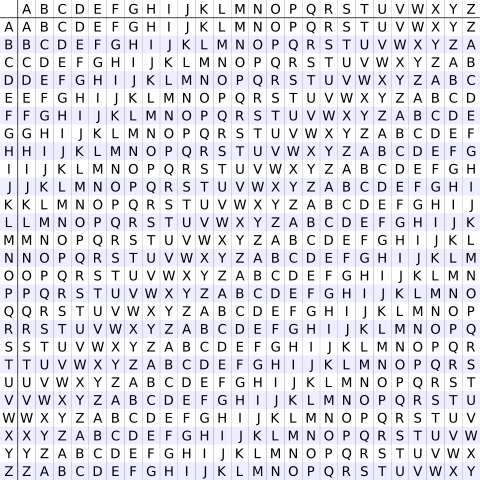
\includegraphics[width=.8\textwidth]{imagens/tabula-recta.png}
  \caption{Tabula Recta}
  \label{fig:tabula-recta}
\end{figure}


\begin{example}
  Considere a seguinte mensagem criptografada com a chave {\tt senha} usando a cifra de Vigenère:

\begin{verbatim}
Mensagem: transparenciapublicaopacidadeprivada
Chave:    senhasenhasenhasenhasenhasenhasenhas
Cifra:    LVNUSHEELNUMNWUTHVJAGTNJIVEQKPJMIHDS
\end{verbatim}  
\end{example}

Para fechar o capítulo vamos fazer o exercício de formalizar a cifra de Vigenère.
A chave consiste em uma sequência de letras, tipicamente escolhidas em um dicionário, mas vamos aqui supor que a escolha seja aleatória e com um tamanho fixado $l$.
A partir dessa semente, podemos gerar uma chave auxiliar $k'$ obtida repetindo $k$ quantas vezes forem necessárias até que $|k'| = |m| = n$.
Para criptografar basta desolcar $m_i$ por $k_i'$ posições.
Formalmente temos que $\Pi = \langle Gen, E, D \rangle$

\begin{itemize}
\item $Gen := k \leftarrow \mathbb{Z}_{26}^l$
\item $E(k, m) = [m_0 + {k_0}'\ mod\ 26] \dots [m_n + {k_n}'\ mod\ 26]$
\item $D(k, c) = [c_0 - {k_0}'\ mod\ 26] \dots [c_n - {k_n}'\ mod\ 26]$
\end{itemize}

\section{Maquinas de Criptografar}
\label{sec:maquinas}

No final da primeira década do século XX foram inventadas as primeiras máquinas de criptografar.
A componente principal dessas {\em maquinas eletromecânicas} é um conjunto de {\em rotores}.
A configuração inicial dos rotores contém a chave da criptografia.
Cada vez que o operador pressiona uma tecla o rotor embaralha as letras.
Dessa forma, essas {\em máquinas rotoras} se comportam como uma sofisticada cifra polialfabética.
Para descriptografar a mensagem, o operador precisa ajustar a máquina em modo de descriptografia, ajustar a configuração inicial com a chave secreta e digitar o texto cifrado.
A máquina então irá se rearrajar para produzir o texto original quando digitado.

As máquinas rotora mais conhecida são da série {\em Enigma}.
Elas foram criadas por um inventor alemão no final da primeira guerra mundial e versões mais modernas foram extensamente usadas durante a segunda guerra pelo exército nazista.
As versões mais simples da máquina possuiam três rotores capazes de gerar $26^3$, ou cerca de $175$ mil possíveis configurações iniciais.
Além disso, era possível trocar a ordem dos rotores multiplicando por $6$ o número de combinações possíveis e chegando a um total de cerca de $105$ mil possibilidades.
A versão utilizada pelo exercito nazista, porém, permitia cerca de $150$ trilhões de possibilidades.
Em 1939 Alan Turing desenvolveu uma máquina eletromecânica chamada {\em Bombe} capaz de decifrar algumas cifras de máquinas Enigma com 3 rotores e, posterioirmente foi melhorada para decifrar mensagens de máquinas Enigma mais sofisticadas.

A história da computação esbarra na história da criptografia neste ponto.
Poucos anos antes da guerra, Alan Turing demonstrara que a satisfatibilidade da lógica de primeira ordem é um {\em problema indecidível}.
Para tanto ele propôs um {\em modelo computacional} que hoje chamamos de {\em Máquinas de Turing}.
Diferente dos modelos computacionais anteriores como o {\em cálculo lambda} de Church ou as {\em funções recursivas} de Gödel, o modelo de Turing era intuitivo.
Além disso, Turing mostrou que era possível construir com seu modelo uma {\em Máquina Universal} capaz de simular qualquer outra Máquina de Turing.
Esse resultado magnífico é o que dá origem a computação.
O primeiro modelo de computador desenvolvido por Turing e sua equipe em Bechley Park foi batizado de {\em Colossus} e tinha como principal propósito quebrar outra cifra usada pelos nazistas durante a guerra, a {\em cifra de Lorenz}.
A cifra de Lorenz é uma versão do que estudaremos com o nome de {\em cifra de fluxo}.
Para decifrar os códigos das máquinas Enigma e da cifra de Lorenz os ingleses tiveram que contar, não apenas com o texto criptografado que interceptavam sem grandes dificuldades, mas também com uma série cifras cujas mensagens eles conheciam previamente.
Veremos mais pra frente a importância desta informação. 
A capacidade dos aliados de decifrar as mensagens de seus adversários foi central para sua vitória. 

O começo do século XX marcou o surgimento das primeiras máquinas de criptografar, as primeiras máquinas de criptoanálise. 
Na metade do século começaram a surgir os primeiros computadores.
Nos anos 70 a comunicação seria revolucionada pelo advento da internet, mas antes disso já ficara claro que era necessário compreender melhor o que faz uma cifra ser segura. 
\chapter{Criptoanálise}
\label{cha:criptoanalise}

Nos capítulos anteriores vimos uma série de cifras que a história deu conta de mostrar que não são seguras.
Neste capítulo focaremos nas técnicas para quebrar essas cifras.
O estudo e a análise dos sistemas de informação com a intenção de desvelar seus segredos é o que chamamos de {\em criptoanálise}.

\section{Ataques Força Bruta}
\label{sec:forca-bruta}

Uma forma universal de quebrar uma cifra é conhecido como {\em ataque força bruta}.
Ele consiste no seguinte procedimento.
O adversário utiliza o esquema $D$, que sempre assumimos ser de conhecimento público, numa cifra $c$ com uma primeira tentativa de chave $k_0$ para produzir $D(k_0, c) = m_0$.
A mensagem $m_0$ provavelmente não fará nenhum sentido, então o adversário repete o processo com uma outra chave $k_1$ e em seguida com $k_2$ e assim por diante até que mensagem produzida seja coerente.

Consideremos a cifra de deslocamento.
Estabelecemos que uma chave nesse tipo de sistema é escolhida aleatoriamente no conjunto $\mathbb{Z}_{26}$.
Assim existem exatamente 26 possibilidades de chave, porque $|\mathbb{Z}_{26}| = 26$.
O número esperado de tentativas até se encontrar a chave procurada é $\frac{|K|}{2}$, neste caso 13.
Ou seja, a cifra de deslocamento é muito vulnerável a ataques de força bruta porque seu universo de chaves é extremamente pequeno.

Em contraste vamos calcular o universo de chaves da cifra de substituição.
Vimos que o universo das chaves de uma cifra de susbstituição é $Perm(\mathbb{Z}_{26})$.
Calcular $|Perm(\mathbb{Z}_{26})|$ é um exercício simples de {\em análise combinatória}.

\begin{eqnarray*}
  |Perm(\mathbb{Z}_{26}|) & = & 26!\\
                         & = & 26.25.24 \dots 1\\
                         & \approx & 4.10^{26}\\
                         & \approx & 2^{88}
\end{eqnarray*}

O universo de chaves na cifra de deslocamento é tão pequeno que é possível testar na mão todas as possibilidades de chaves.
Certamente não é possível testar as possibilidades de chaves da cifra de substituição na mão.
Ataques força bruta, porém, são facilmente automatizáveis.
Voltaremos a pergunta sobre o tamanho do universo de chaves para uma comunicação segura no capítulo \ref{chap:senhas}.


\begin{example}
Muitos dos roteadores modernos possuem um mecanismo chamado de WPS (Wi-Fi Protected Setup) que supostamente simplificaria o processo de conexão, especialmente na configuração do hardware.
O WPS permite que um usuário se conecte remotamente e sem fio no roteador desde que possua um PIN (Personal Identification Number).
Esse PIN é uma sequência de oito digitos de 0 a 9.
Ou seja, o universo das chaves é $10^8 \approx 2^{27}$.
Neste contexto, um ataque força-bruta é possível e toma entre 4 e 8 horas.  
\end{example}


\section{Ataques de Frequência}
\label{sec:frequencia}

A cifra de substituição é suficientemente segura contra ataques de força-bruta.
Como vimos, porém, ela não é tão segura quanto a rainha Mary da Escócia gostaria.
A forma como os funcionários da rainha Elizabeth quebraram a cifra de substituição é o que chamamos de {\em ataque de frequência}.
A ideia por trás desse tipo de ataque é bastante simples.
Na cifra de substituição, cada letra é substituída por um símbolo.
Portanto, a frequência de cada símbolo em um texto suficientemente longo deve ser parecida com a frequência média de cada letra naquela língua.
Por exemplo, no português, esperamos que os símbolos mais comuns sejam o {\tt a}, o {\tt e} e o {\tt o}.
Para piorar -- ou melhorar dependendo da perspectiva -- na maioria das línguas há digrafos particulares, por exemplo, no português dois símbolos repetídos provavelmente representam o {\tt r} ou o {\tt s} e o {\tt h} quase sempre vem depois do {\tt l} ou do {\tt n}.
Se o texto a ser decifrado for suficientemente longo, essas pistas podem ser suficientes para quebrar a cifra.

No seguinte trecho de ``O escaravelho de ouro'' de Edgar Allan Poe a personagem descreve essa técnica que ela utilizou para decifrar um texto em inglês \cite{}:

\begin{quote}
``Ora, no inglês, a letra que ocorre com mais frequência é a letra {\tt e}. 
Depois dela, a sucessão é: {\tt a o i d h n r s t u y c f g l m w b k p q x z}. 
O e prevalece de tal maneira que quase nunca se vê uma frase isolada em que ele não seja predominante. 
Aqui nós temos, portanto, bem no início, uma base que permite mais do que um mero palpite. 
O uso que se pode fazer da tabela é óbvio, mas, neste criptograma em particular, não precisamos nos valer dela por inteiro. 
Como nosso caractere dominante é o {\tt 8}, começaremos assumindo que este é o {\tt e} do alfabeto normal. (...)''
\end{quote}

Em português, faz sentido separar as letras em cinco blocos, com frequência de ocorrência decrescente:
\begin{enumerate}
\item {\tt a}, {\tt e} e {\tt o}
\item {\tt s}, {\tt r} e {\tt i}
\item {\tt n}, {\tt d}, {\tt m}, {\tt u}, {\tt t} e {\tt c}
\item {\tt l}, {\tt p}, {\tt v}, {\tt g}, {\tt h}, {\tt q}, {\tt b} e {\tt f}
\item {\tt z}, {\tt j}, {\tt x}, {\tt k}, {\tt w} e {\tt y}
\end{enumerate}

\section{Ataques à ``Cifra Invencível''}
\label{sec:criptoanalise-vegenere}

Apesar da fama de ``inquebrável'' que a cifra de Vigenère oustentou até o começo do século XX, desde a metade do século anterior já eram conhecidos métodos de criptoanálise capazes de detorratar esse tipo de cifra.
Em 1854 John Hall Brock Thwaites submeteu um texto cifrado utilizando uma cifra supostamente por ele inventada.
Charles Babbage, o inventor das máquinas que precederam o computador moderno, mostrou que no fundo a cifra de Thwaites era equivalente a cifra de Vigenère.
Após ser desafiado, Babbage, decifrou uma mensagem criptografada por Thwaites duas vezes com chaves diferentes.

Em 1863 Friedrich Kasiski formalizou um ataque contra a cifra de Vigenère que ficou conhecido como {\em teste de Kasiski}.
O ataque considera o fato de que a chave se repete com uma frequência fixa e, portanto, há uma probabilidade de produzir padrões reconhecíveis.
Considere o exemplo extraído da Wikipédia:

\begin{example}
\begin{verbatim}
Mensagem: cryptoisshortforcryptography
Chave:    abcdabcdabcdabcdabcdabcdabcd
Cifra:    CSASTPKVSIQUTGQUCSASTPIUAQJB
\end{verbatim}  
\end{example}

Note que o padrão CSASTP se repete na cifra.
Isso ocorre porque o prefixo {\tt crypto} foi criptografado com a mesma chave.
Uma vez encontrado um padrão como este, é calculada a distância entre as repetições.
Neste caso a distância é 16, o que significa que o tamanho da chave deve ser um divisor de 16 (2, 4, 8 ou 16).
Com esta informação, podemos aplicar um ataque de frequência nos caracteres de 2 a 2, de 4 a 4, de 8 a 8 e de 16 a 16.

\section{Exercícios}
\label{sec:exercicios}


\begin{exercicio}
Calculo o tamanho do universo das chaves em uma cifra de Vigenère da forma como usada normalmente (escolhendo um palavra) e na forma como apresentamos formalmente (sequência aleatória com tamanho fixo $l$)?  
\end{exercicio}


\begin{exercicio}
Construa um script que extraia um corpus do português moderno (por exemplo, textos da wikipedia) e calucule a frequência de ocorrência das letras do alfabeto. 
\end{exercicio}

\begin{exercicio}
Em 2017 um rapaz que ficou conhecido como menino do Acre ficou dias desaparecido e deixou uma serie de livros criptografados com cifra de substituição em seu quarto.
A Figura \ref{fig:menino-do-acre} está reproduzida uma página de um desses livros. 
Utilize a análise de frequência para decifrar o texto.
\end{exercicio}

\begin{figure}[htbp]
  \centering
  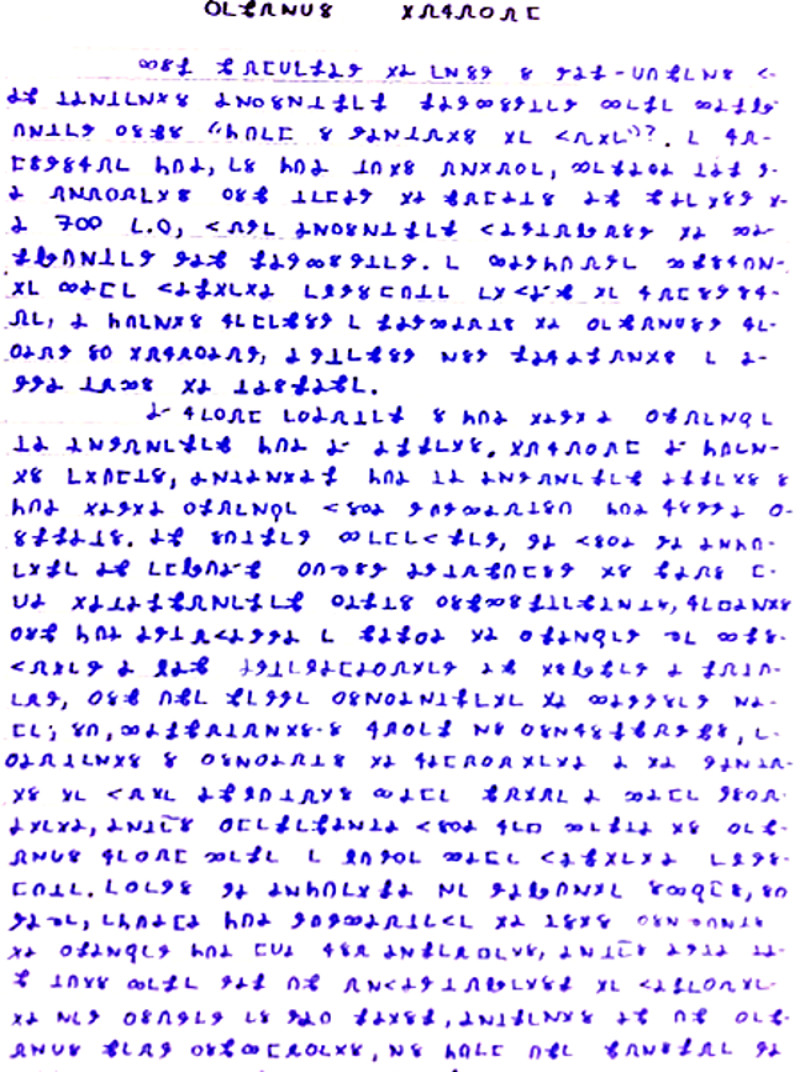
\includegraphics[width=.8\textwidth]{imagens/bruno.jpg}
  \caption{Texto criptografado pelo Menino do Acre}
  \label{fig:menino-do-acre}
\end{figure}

% Colocar aqui a frequência das letras em portugês, de preferência com um gráfico
% Inserir o exemplo do menino do Acre a partir do trabalho que eles enviarem
% Técnica para quebrar a cifra de Vigenère


\chapter{Sigilo Perfeito}
\label{cha:sigilo-perfeito}

No final dos anos 40, com o desenvolvimento dos primeiros computadores e a experiência da quebra das cifras mecanicamente produzidas por poderosas máquinas desenvolvidas pelo esforço de guerra do nazismo, alguns cientístas se voltaram para um problema central no campo da criptografia: o que torna um sistema de criptografia seguro?
As cifras que vimos até agora são conhecidas como ``cifras clássicas'' extamente porque elas precedem desse debate moderno, e não a toa foram todas derrotadas cedo ou tarde.
Informalmente, poderíamos dizer que o problema dos esquemas clássicos de criptografia é que eles guardam muita informação sobre a mensagem (frequência das letras, dos dígrafos, letras duplas etc.). 
Não é uma coincidência, portanto, que a primeira tentativa de formalizar o conceito de segurança tenha sido proposto por Claude Shannon, o fundador da teoria da informação.
Shannon definiu o que hoje chamamos de {\em sigilo perfeito}.
Um esquema de criptografia garante o sigilo perfeito se a cifra não guarda nenhuma informação sobre a mensagem que a gerou.
Ou, de maneira um pouco mais descritiva, se a probabilidades da cifra ocorrer é independente da probabilidade da mensagem:

\begin{definition}
  Um esquema de criptografia simétrica $\Pi = \langle Gen, E, D \rangle$ garante o {\em sigilo perfeito} se, supondo que $Pr[C=c] > 0$, para toda distribuição de probabilidade sobre $M$ temos que:
\begin{displaymath}
  Pr[M = m | C = c] = Pr[M = m]
\end{displaymath}

Ou de maneira equivalente se para todo $m_0, m_1 \in M$ e todo $c \in C$ temos que:
\begin{displaymath}
  Pr[C = c | M = m_0] = Pr[C = c | M = m_1]
\end{displaymath}
\end{definition}

Essa segunda formulação é mais intuitiva, ela estabelece que um sistema garante o sigilo perfeito se a probabilidade de $m_0$ produzir a cifra $c$ é idêntica a probabilidade de qualquer outra mensagem $m_1$ produzir a mesma cifra $c$.
O exemplo a seguir mostra que a cifra de substituição não garante o sigilo perfeito:

\begin{example}
  Seja $\Pi = \langle Gen, E, D \rangle$ o sistema de criptografia de substituição e sejam $c = \textrm{\tt ANA}$, $m_0 = \textrm{\tt OVO}$ e $m_1 = \textrm{\tt EVA}$.
Como o sistema $\Pi$ substitui cada letra da mensagem por uma letra na cifra, existem chaves $k$ tal que $E(k, m_0) = c$ -- basta que $k(\textrm{\tt O}) = \textrm{\tt A}$ e $k(\textrm{\tt V}) = \textrm{\tt N}$, de fato a chance de escolher uma chave assim é $\frac{1}{26^2} = \frac{1}{676}$ --, mas não existe nenhuma chave $k'$ tal que $E(k', m_1) = c$.
Portanto temos que:
\begin{displaymath}
Pr[C = c | M = m_0] =  \frac{1}{676} \neq Pr[C = c | M = m_1] = 0  
\end{displaymath}
\end{example}

Uma forma equivalente, e útil como veremos mais para frente, de definir sigilo perfeito é a partir de um jogo.
Imaginamos que há um adversário $\mathcal{A}$ cujo objetivo é quebrar a cifra produzida pelo sistema $\Pi$.
O jogo funciona da seguinte maneira: $\mathcal{A}$ escolhe duas mensagens $m_0$ e $m_1$ com o mesmo tamanho ($|m_0| = |m_1|$) e envia para o sistema $\Pi$.
O sistema gera uma chave $k$ usando o algoritmo $Gen$ e sorteia aleatoriamente uma das mensagens para criptografar ($\Pi$ sorteia $b \leftarrow \{0, 1\}$ e criptografa $m_b$).
A cifra produzida $E(k, m_b) = c$ e enviada de volta para o adversário, cujo desafia é acertar qual das duas mensagens foi cifrada.
O diagrama abaixo ilustra o processo:

\begin{center}
\begin{tikzpicture}[node distance=2cm,auto,>=latex]
\tikzset{
  player/.style={draw,shape=rectangle,rounded corners,minimum width=4em,minimum height=6em}
}
\node[player] (system) {$\Pi$};
\node[player] (adversary) at (10,0) {$\mathcal{A}$};
\draw[->] (9,.5) -> node[above]{$m_0, m_1 \in M : |m_0| = |m_1|$} (1,.5);
\draw[->] (1,-.5) -> node[above]{$E(k,m_b) = c$} (9,-.5);
\draw[->] (0,2) -> node{$b \leftarrow \{0,1\}$} (system);
\draw[->] (adversary) -> node{$b' \in \{0,1\}$} (10,-2);
\end{tikzpicture}
\end{center}

Chamamos o experimento ilustrado pelo diagrama de $PrivK^{eav}_{\Pi, \mathcal{A}}$.
Os subscritos indicam que o experimento depende do sistema $\Pi$ e do adversário $\mathcal{A}$.
O resultado do experimento deve ser $0$ se o adversário perdeu o desafio e $1$ caso contrário.
Formalmente temos que:
\begin{displaymath}
  PrivK^{eav}_{\Pi, \mathcal{A}} = \left\{
    \begin{array}{lcl}
      1 & \textrm{se} & b = b'\\
      0 & \textrm{c.c.} &\\
    \end{array}
    \right.
\end{displaymath}

É possível provar que um sistema $\Pi$ garante o {\em sigilo perfeito} se e somente se para qualquer adversário $\mathcal{A}$ temos que:
\begin{displaymath}
Pr[PrivK^{eav}_{\Pi, \mathcal{A}} = 1] = \frac{1}{2}
\end{displaymath}

Em palavras, o sistema possui sigilo perfeito se nenhum adversário é capaz de acertar qual ads mensagens produziu a cifra $c$ com probabilidade melhor do que um meio.

\section{One Time Pad}
\label{sec:otp}

Temos agora uma definição formal de segurança.
Vimos que a cifra de substituição não satisfaz essa definição, mas na verdade nenhuma das cifras clássica a satisfaz.
Não seria desejável que essas cifras satisfizessem a definição, pois vimos no capítulo anterior que nenhuma das cifras clássicas é segura e todas podem ser derrotadas se o adversário tiver acesso a uma cifra de tamanho suficientemente grande.
Ficamos então com o desafio de encontrar algum sistema que satisfaça essa definição, caso tal sistema exista.

No que segue apresentaremos um sistema chamado {\em One Time Pad} (OTP), também conhecida como {\em cifra de Vernan}, e mostraremos que ele garante o sigilo perfeito.
A partir deste ponto, conforme começaremos a investigar sistemas a serem implementados computacionalmente, consideraremos que o espaço $M$ das mensagens (assim como o espaço $C$ das cifras) será representado como sequências de bits.
No caso específico do OTP assumiremos que as mensagens e a cifras possuem um tamanho fixo $n$.
Mais importante é o fato de que o universo das chaves é também um conjunto de sequências de bits do mesmo tamanho.
Assim temos que $M = C = K = \{0,1\}^n$.
O sistema $\Pi = \langle Gen, E, D \rangle$ é definido pelos seguintes algoritmos:
\begin{itemize}
\item $Gen := k \leftarrow \{0,1\}^n$
\item $E(k,m) = [m_0 + k_0\ mod\ 2] \dots [m_n + k_n\ mod\ 2] = m \xor k$
\item $D(k,c) = [c_0 + k_0\ mod\ 2] \dots [c_n + k_n\ mod\ 2] = c \xor k$
\end{itemize}

Para verificar a corretude do sistema basta notar que:

\begin{eqnarray*}
  D(k, E(k, m)) & = & D(k, k \xor m)\\
                & = & k \xor (k \xor m)\\
                & = & (k \xor k) \xor m\\
                & = & m
\end{eqnarray*}

A derivação usa o fato de que a operação de {\em ou exclusivo} $\xor$ é associativa, que $x \xor x = 1$ e $1 \xor x = x$ para todo sequência de bits $x \in \{0,1\}^*$.
Deixamos como exercício mostrar essas três propriedades da operação.

\begin{example}
  Considere uma mensagem $m = 101010$ e uma chave $k = 010001$.
Usando o sistema One Time Pad a cifra produzida é a seguite:

\begin{displaymath}
  \begin{array}{ccccc}
    m & \xor & k & = & c \\
    101010 & \xor & 010001 & = & 111011
  \end{array}
\end{displaymath}
\end{example}

Como antecipado, é possível, e relativamente simples provar que o OTP possui sigilo perfeito.

\begin{theorem}
  O sistema de criptografia {\em One Time Pad} possui sigilo perfeito.
\end{theorem}

\begin{proof}
  Seja $K = M = C = \{0,1\}^n$.
  Dada uma cifra $c \in C$ e uma mensagem qualquer $m \in M$, existe uma única chave $k \in K$ tal que $E(k,m) = c$.
  A chave é exatamente $k = m \xor c$, pois:
  
  \begin{eqnarray*}
    E(k, m) & = & k \xor m \\
            & = & (m \xor c) \xor m\\
            & = & (m \xor m) \xor c\\
            & = & c
  \end{eqnarray*}

Como existe exatamente uma chave possível que faz com que $E(k,m) = c$, temos que a probabilidade se produzir $c$ dado uma mensagem qualquer $m$ é igual a probabilidade de sortear uma chave específica no universo $K = \{0,1\}^n$ que é $\frac{1}{2^n}$:
\begin{displaymath}
  Pr[C = c | M = c] = \frac{1}{2^n}
\end{displaymath}

Essa probabilidade é idêntica para qualquer $m \in M$.
Portanto, temos que $Pr[C = c| M = m_0] = Pr[C = c | M = m_1] = \frac{1}{2^n}$. 
\end{proof}

O {\em One Time Pad} possui duas severas limitações.
A primeira é indicada pelo próprio nome do sistema.
A sistema supõe que a chave de criptografia $k$ seja usada exatamente uma vez (``one time'').
Caso o mesmo $k$ seja usada para criptografar duas mensagens distintas $m_1$ e $m_2$, o sistema se torna completamente inseguro.

Para ilustrar essa limitação considere que duas cifras $c_0$ e $c_1$ foram produzidas usando a mesma chave $k$.
Assim temos que $c_0 = k \xor m_0$ e $c_1 = k \xor m_1$.
Note o que acontece quando aplicamos o ou exclusivo entre as duas cifras eliminamos a chave:


\begin{eqnarray*}
  c_0 \xor c_1 & = & (k \xor m_0) \xor (k \xor m_1)\\
              & = & (k \xor k) \xor (m_0 \xor m_1)\\
              & = & m_0 \xor m_1
\end{eqnarray*}

Uma vez eliminada a chave, é fácil separar as mensagens $m_0$ de $m_1$ utilizando um técnica similar ao ataque de frequência.

A segunda e mais crítica limitação do OTP é o tamanho de sua chave.
A suposição que fizemos é que o tamanho da chave deve ser tão grande quanto a mensagem a ser cifrada.
Há uma série de problemas práticos com isso.
Computacionalmente não é possível gerar chaves aleatórias muito grandes, o que limita o tamanho das mensagens que podemos cifrar.
Além disso, assumimos que as chaves são compartilhadas entre as partes.
Deixamos os detalhes sobre a distribuição de chaves para o capítulo \ref{}, mas por ora podemos adiantar que se nossa chave é tão grande quanto a mensagem, porque não enviamos a mensagem pelo mesmo canal que enviaríamos a mensagem?
Enfim, um sistema cuja a chave seja tão grande quanto a mensagem é de muito pouca utilidade prática.

Encerramos este capítulo mostrando que esta segunda limitação do OTP infelizmente não é uma peculiaridade do sistema.
Na verdade todo sistema que possua sigilo perfeito está fadado a ter chaves tão grandes o maiores do que a mensagem.
Esse resultado negativo foi proposto e demonstrado pelo próprio Shannon ainda nos anos 40.


\begin{theorem}[Teorema de Shannon]
Seja $\Pi = \langle Gen, E, D \rangle$ um sistema que garante o sigilo perfeito, então temos que $|K| \geq |M|$.  
\end{theorem}
\begin{proof}
  Consideraremos $M(c)$ como o conjuto de todas as mensagens que podem produzir $c$, ou seja, as mensagens $m \in M$ tal que $E(k, m) = c$ para algum $k \in K$.
  É claro que $|M(c)| \leq |K|$.
  Agora suponha por absurdo que $|K| < |M|$.
  Neste caso existiria uma mensagem $m \notin M(c)$ e, portanto, $Pr[M = m] \neq 0$.
  Mas, por definição, temos que $Pr[C = c | M = m] = 0$ contradizendo a hipótese deu que $\Pi$ garante o sigilo perfeito. 
\end{proof}

A definição de Shannon foi a primeira tentativa séria de definir segurança de sistemas de criptografia, mas o próprio autor da definição foi capaz de demonstrar suas limitações.
Nos próximos capítulos apresentaremos definições de segurança mais fracas e mais úteis para nossos propósitos.

\section{Exercício}
\label{sec:exercicio}

\begin{exercicio}
  Mostre que o $1$ é elementro neutro na operação $\xor$, ou seja, que para todo $x \in \{0,1\}^*$ temos que $x \xor 1 = 1 \xor x = x$.
\end{exercicio}

\begin{exercicio}
  Mostre que a operação $\xor$ é {\em associativa}, ou seja, que para todo $x,y,z \in \{0,1\}^*$ temos que $x \xor (y \xor z) = (x \xor y) \xor z$.
\end{exercicio}

\begin{exercicio}
  Mostre que a operação $\xor$ é {\em comutativa}, ou seja, que para todo $x,y \in \{0,1\}^*$ temos que $x \xor y = x \xor y$.
\end{exercicio}

\begin{exercicio}
  Mostre que para qualquer sequência de bits $x \in \{0,1\}^*$ temos que $x \xor x = 1$.
\end{exercicio}

\begin{exercicio}
  Mostre que a cifra de deslocamento não garante sigilo perfeito.
\end{exercicio}


\chapter{Criptografia Moderna}
\label{cha:criptografia-moderna}

No capítulo anterior apresentamos uma primeira tentativa de definir formalmente segurança de sistemas de criptografia.
A definição, proposta por Shannon, estabelece que um sistema garante o {\em sigilo perfeito} se a cifra não guarda nenhuma informação da mensagem que a produziu.
No final do capítulo, porém, vimos que esta definição não é muito útil na prática, pois obriga o universo de chaves ser pelo menos tão grande quanto o universo das mensagens.

Apesar do fracasso desta primeira tentativa de formalizar o conceito de segurança, não abandonaremos a ideia geral.
A abordagem da {\em criptografia moderna}, que utilizaremos nesta apostila, segue três princípios básicos:
\begin{enumerate}
\item {\em definições formais:} As noções de segurança utilizadas serão apresentadas de maneira formal por meio de definições. 
As definições prévias nos ajudam a comparar sistemas e avaliar sua segurança a partir de critérios estabelecidos previamente.
\item {\em suposições precisas:} Na maioria dos casos seremos forçados a fazer suposições sobre os sistemas de criptografia que não seremos capazes de demonstrar.
Ainda assim, é imprescindível explicitar essas suposições de maneira clara e formal.
Nossa incapassidade de provar tais suposições não nos impede de validá-las empiricamente.
Grande parte do trabalho envolvido na criptografia moderna consiste em validar testar as suposições sobre um sistema e buscar suposições mais simples e básicas.
\item {\em demonstrações formais:} Quando somos capazes de formalizar nossas suposições e a definição de segurança desejada, eventualmente podemos demonstrar que um sistema que satisfaz as suposições garante determinada noção de segurança.
Esse tipo de demonstração reduz o problema da segurança às suposições do sistema que devem ser mais simples e mais fáceis de validar empiricamente.
Esta redução permite que se substitua um sistema cuja suposição foi falseada antes que ele seja quebrado.
\end{enumerate}

As definições de segurança em geral possuem dois componentes: uma garantia de segurança -- o que pode ser considerado um ataque bem sucedido -- e um modelo de ameaças.
Por exemplo, na definição de {\em sigilo perfeito} a garantia de segurança é que nenhuma informação sobre a mensagem esteja contida na cifra -- ou como formulamos, a probabilidade de ocorrência da cifra deve ser independente da probabilidade de ocorrência da mensagem -- e o modelo de ameaça assume que o adversário tem acesso apenas ao texto cifrado e nada mais. 
Os modelos de ameaças que estudaremos no livros incluem:
\begin{itemize}
\item {\em ataque ciphertext-only:} Este é o modelo assumido na definição de sigilo perfeito.
Nele assumimos que o adversário tem acesso apenas a um texto cifrado de tamanho arbitrário.
\item {\em ataque chosen-plaintext:} Neste modelo, além de assumir que o adversário tem acesso à cifra, assumimos que ele é capaz de escolher uma quantidade de mensagens e verificar como elas seriam cifradas pelo sistema.
\item {\em ataque chosen-ciphertext:} Neste modelo assumimos que o adversário é também capaz de escolher certas cifras e verificar como elas seriam decifras pelo sistema.
\end{itemize}

Essas definições são progressivamente mais fortes, ou seja, assumem progressivamente maior capacidade de ataque do adversário.
Note que nossos modelos de ataque não fazem qualquer suposição sobre a estratégia utilizada pelo adversário.
Em geral, a definição mais adequada depende das necessidades do problema em mãos -- eventualmente pode ser desejável um sistema mais fraco e mais eficiente.

Nossa primeira tentativa de definir segurança esbarrou na limitação inconveniente expressa pelo teorema de Shannon.
Afirmamos no capítulo anterior que o sigilo perfeito pode ser definido por meio de um jogo.
O sigilo perfeito é garantido se nenhum adversário for capaz de distinguir qual mensagem foi encriptada pelo sistema.
Para contornar as limitações expressas pelo teorema de Shannon, enfraqueceremos este tipo de definição de duas formas:
\begin{itemize}
\item O adversário deve ser {\em eficiente} e usar sua estratégia em um tempo razoável.
  Ou seja, eventualmente um adversário pode derrotar o sistema desde que seja dado a ele tempo suficiente.
  A existência de um adversário como este não violará nossa definição de segurança, pois não traz uma real ameaça na prática.
\item O adversário pode eventualmente derrotar o sistema, mas com uma {\em probabilidade muito pequena}.
Colocado de outra maneira, a cifra pode guardar alguma informação sobre a mensagem desde que seja muito pouca. 
\end{itemize}

\section{Abordagem Assintótica}
\label{sec:abord-assint}

Em termos práticos o que buscamos uma noção de segurança em que para um adversário ter sucesso ele precisaria rodar seu algoritmo em uma máquina excelente por um intervalo bem grande de tempo.
Alternativamente esperamos que eventualmente o adversário derrote o sistema em pouco tempo, mas com uma probabilidade muito baixa.
O problema com essa abordagem é como definir o que seria uma ``máquina excelente'', uma ``intervalo bem grande de tempo'' e uma ``probabilidade muito baixa''.
Essas questões são particularmente complicados em um contexto em que a capacidade computacional evolui de maneira acelerada.

Ao invés de estabelecer valores fixos para definir esses limites, partiremos de uma {\em abordagem assintótica}.
Suporemos que o algoritmo de geração de chaves $Gen$ recebe um {\em parâmetro de segurança} $n$ e estabeleceremos nossos limites em função deste parâmetro -- tipicamente denotaremos esse valor usando a notação unária $1^n$, pois a tempo de execução costuma ser calculado como uma função do tamanho da entrada.
Para os efeitos desta apostila podemos assumir que o parâmetro está relacionado ao tamanho da chave a ser gerada e que é de conhecimento público.
O parâmetro de segurânça permite que as partes ajustem seu sistema para o nível desejado de segurança -- aumentar seu tamanho costuma refletir em um aumento no tempo de processamento do sistema e em um aumento no tamanho da chave, portanto, quem projeta o sistema tem um incentivo para querer minimizá-lo as custas de diminuir sua segurança.
A capacidade de ajustar o parâmetro de segurânça possui grandes vantagens práticas, pois permite se defender de adversários com poder computacional mais forte com o passar do tempo. 

Vamos estabelecer que o adversário buscará quebrar a cifra usando um algorítmo randomizado polinomial em $n$ e que ele pode vencer com uma probabilidade desprezível em $n$.
A suposição de que o adversário usa um algoritmos randomizado é forte, significa que ele é capaz de acessar uma quantidade arbitrária de bits aleatórios.
Isso certamente não é possível na prática, mas serve bem aos propósitos de uma análise de pior caso.
Já a probabilidade ser desprezível significa que ela cresce assintoticamente mais devagar do que o inverso de qualquer polinômio.
Formalmente, $\varepsilon: \mathbb{N} \to \mathbb{N}$ é {\em desprezível} se para todo polinômio $p$ existe um número positivo $N$ tal que para todo $n > N$ temos que $\varepsilon(n) < \frac{1}{n}$.

Estamos agora em condições de reescrever a definição de segurança formalmente incorporando os enfraquecimentos descritos neste capítulo.

\begin{definition}
  Considere o jogo apresentado no Capítulo \ref{cha:sigilo-perfeito}, um sistema $\Pi = \langle Gen, E, D \rangle$ é seguro contra ataques {\em ciphertext-only} se para todo adversário polinomial $\mathcal{A}$ existe uma função desprezível $\varepsilon$ tal que para todo $n$:
\begin{displaymath}
  Pr[PrivK^{eav}_{\Pi, \mathcal{A}}(n) = 1] \leq \frac{1}{n} + \varepsilon(n)
\end{displaymath}
\end{definition}

Lembrando que agora o algoritmo $Gen$ recebe como o parâmetro de segurança $n$ em notação unária para gerar a chave de tamanho apropriado.
Em palavras, a definição estabelece que um sistema é seguro contra ataques {\em ciphertext-only} se nenhum algoritmo eficiente é capaz de derrotá-lo com probabilidade consideravelmente maior do que $\frac{1}{2}$.
Resta mostrar um sistema que satisfaça essa definição.


\section{Exercícios}
\label{sec:exercicios}


\begin{exercicio}
  Sejam $\varepsilon_1$ e $\varepsilon_2$ duas funções desprezíveis. 
  Mostre que $\varepsilon_1 + \varepsilon_2$ é desprezível.
\end{exercicio}

\begin{exercicio}
  Seja $\varepsilon$ uma função desprezível e $p$ um polinômio. 
  Mostre que $p\varepsilon$ é desprezível.
\end{exercicio}
\chapter{Cifras de Fluxo}
\label{cha:cifras-de-fluxo}

No capítulo anterior apresentamos uma definição formal para segurança contra ataques em que o adversário tem acesso apenas ao texto cifrado.
Neste capítulo vamos apresentar uma forma de construir um sistema que satisfaz essa definição.
A ideia geral da construação é a seguinte: partimos de uma sequência aleatória de bits chamado de {\em semente} e a partir dela geramos uma sequência maior de bits a ser usada para encriptar a mensagem usando o ou exclusivo como no OTP.
Apesar desta sequência ser gerada de maneira determinística, a segurança do sistema depende do fato de que ela se pareça aleatória.
Informalmente, um {\em gerador de números pseudoaleatórios} (PRG) é essa função que recebe uma semente aleatória e a expande em uma sequência com cara de aleatória.

Sistemas de cifra de fluxo foram estudados extensamente nos anos 80.
A abordagem para verificar se o gerador de números pseudoaleatórios é suficientemente forte consistia em aplicar uma série de testes estatísticos na sequência gerada para tentar distinguí-lo de uma sequência aleatória.
Assim, por exemplo, um teste pode verificar se a probabilidade de o primeiro bit da sequência ser igual $1$ é $\frac{1}{2}$ ou que a probabilidade de ocorrência de pelos menos três $0$s em qualquer subsequência de tamanho $4$ deve ser $\frac{5}{16}$ -- existem uma sequência em que o $0$ ocorre quatro vezes e mais quatro sequências possíveis em que ele ocorre três vezes.
Um teste como recebe uma sequencia produzida por um PRG e deve retornar $1$ se o teste passou e $0$ caso contrário.
O objetivo do teste é distinguir as sequências de bits produzidas por um PRG de uma sequência realmente aleatória.
Por este motivo, esses testes são chamados {\em distinguidores}.

Uma bateria de distinguidores pode ser usada para verificar a qualidade de um PRG.
Idealmente nenhum teste eficiente deveria ser capaz de distinguir o PRG de uma sequência aleatória, ou pelo menos incapaz de fazê-lo com probabilidade considerável.
Definiremos um gerador de números pseudo-aleatórios como um algoritmo $G$ que recebe uma semente $s$ de tamanho $n$ e produz $G(s)$ de tamanho $l(n)$ onde $l$ é um polinômio que define o {\em fator de expansão} do PRG -- quão maior é a sequência produzida em relação a semente -- e tal que nenhum algoritmo polinomial $D$ é capaz de distinguir $G(s)$ de um sequencia $r$ escolhida aleatóriamente em $\{0,1\}^{l(n)}$ com probabilidade não desprezível.
Formalmente temos o seguinte:


\begin{definition}
  Seja $l$ um polinômio e $G$ um algoritmo determinístico polinomial que recebe $s \in \{0,1\}^n$ e retorna $G(s) \in \{0,1\}^{l(n)}$ e seja $r \leftarrow \{0,1\}^{l(n)}$.
  O algoritmo $G$ é um {\em gerador de números pseudo-aleatórios} se:
\begin{enumerate}
\item $l(n) > n$ para todo $n$ e
\item para todo algoritmo polinomial $D$ existe uma função desprezível $\varepsilon$ tal que:
\begin{displaymath}
  |Pr[D(r) = 1] - Pr[D(G(s)) = 1]| \leq \varepsilon(n)  
\end{displaymath}
\end{enumerate}
\end{definition}


\begin{example}
  Considere um algoritmo $G$ que recebe $s \in \{0,1\}^n$ e devolve $0^{l(n)}$.
  Certamente $G$ não é um PRG e podemos mostrar isso com um distinguidor $D$ que recebe $w \in \{0,1\}^{l(n)}$ e devolve $1$ se $w = 0^{l(n)}$ e $0$ caso contrário.
  É fácil ver que para $r \leftarrow \{0,1\}^{l(n)}$ e $s \leftarrow \{0,1\}^n$ temos que $Pr[D(r) = 1] = \frac{1}{2^{l(n)}}$ e $Pr[D(G(s)) = 1] = 1$ e, portanto, temos que:
\begin{displaymath}
  |Pr[D(r) = 1] - Pr[D(G(s)) = 1]| = 1 - \frac{1}{2^{l(n)}}
\end{displaymath}

\end{example}


A restrição de que o distinguidor seja eficiente é extritamente necessária.
Em particular é sempre possível construir um distinguidor usando uma espécie de ataque de força bruta.
Dado uma sequência $w$, o algoritmo $D$ testa todos as possíveis sementes $s$ e verifica se $G(s) = w$ e devolve $1$ caso exista e $0$ caso contrário.
Esse teste é eficaz pois $Pr[D(G(s)) = \frac{1}{2^n}] = 1$, mas $Pr[D(r) = 1] = \frac{1}{2^{l(n)}}$.
Porém, o teste não é eficiente.
De fato $D$ não é polinomial, mas exponencial, pois o tempo esperado para testar todos os valores de $s$ é $2^{n-1}$. 

\section{Linear-Feedback Shift Registers}
\label{sec:lfsr}

A existência de PRGs não foi demonstrada matematicamente.
No capítulo \ref{} mostraremos que a dificuldade associada a este tipo de problema.
A abordagem utilizada em relação a PRG é empírica, ou seja, os candidatos a PRG são empiricamente validados a cada tentativa frustrada de construir um distinguidor empírico para eles.

Assim, na prática utilizamos um par de algoritmos $\langle Init, GenGits \rangle$.
O primeiro algoritmo recebe a semente $s$ como entrada e opcionalmente um vetor inicial $IV$ e devolve um estado inicial $st_0$.
O segundo algoritmo recebe como entrada o estado atual $st_i$, devolve um bit $y$ e atualiza o estado para $st_{i+1}$.
Assim para cada semente, o algoritmo produz um {\em fluxo} infinito de bits -- sendo os $l(n)$ primeiros bits geram $G(s)$.

Um exemplo deste tipo de algoritmo são os chamados {\em Linear-Feedback Shift Registers} (LFSRs).
Um LFSR consiste de um vetor de registradores $s_{n-1} \dots s_0$, que guardam exatamente um bit cada, e uma escolha de um subconjunto desses chamados {\em coeficientes de feedback}.
A cada passo o estado é atualizado deslocando todo vetor uma posição para a direita e produzindo um novo bit que é calculado como o ou esclusivo de todos os registros contidos no coeficiente de feedback.
Para simplificar a notação, podemos imaginar que os coeficientes de feedback são bits $c_{n-1} \dots c_0$ de forma que $c_k = 1$ se a posiação $k$ deve ser usada para gerar o novo bit e $0$ caso contrário.
Assim, o novo bit no registrador $s_{n-1}$ pode ser calculado como $s_{n-1} := \bigoplus_{i=0}^{n-1}c_is_i$.


\begin{example}
  Considere um LFSR com quatro registradores sendo o primeiro e o terceiro parte do coeficiete de feedback.
Se a configuração inicial dos registradores é $\langle 0,0,1,1 \rangle$ os próximos passos são os seguintes:
\begin{displaymath}
  \langle 0,0,1,1 \rangle \vdash
  \langle 1,0,0,1 \rangle \vdash 
  \langle 1,1,0,0 \rangle \vdash
  \langle 1,1,1,0 \rangle \vdash
  \langle 1,1,1,1 \rangle
\end{displaymath}
\end{example}

Um LSFR com $n$ registradores é capaz de gerar no máximo $2^n$ bits até começar a repetir sua sequência.

O único segredo do LFSR são os coeficientes de feedback $c_{n-1} \dots c_0$.
Um ataque relativamente simples a um LFSR consiste em observar os $n$ primeiros bits gerados $y_{n+1} \dots y_{2n}$ e resolver o seguinte sistema linear:

\begin{eqnarray*}
  y_{n+1} &    =   & c_{n-1}y_n \xor \dots \xor c_0 y_1\\
         & \vdots &  \\
  y_{2n}  &    =   & c_{n-1}y_{2n-1} \xor \dots \xor c_0 y_n\\      
\end{eqnarray*}

É possível mostrar que essas equações são linearmente independentes e, portanto, elas determinam unicamente os coefientes.
Uma vez determinados os coeficientes, podemos prever cada novo bit o que torna simples a tarefa de construir um distinguidor para o gerador.

Resumindo, o LFSR não é seguro pois a operação que gera novos bits é linear o que permite que ela seja previsível.
LFSRs não são PRG seguros, mas muitos PRGs nada mais são do que versões alteradas deste esquema geral.
Tipicamente os PRGs usados na prática substituem a operação de ou exclusivo por alguma operação não linear.

Em um concurso científico de 2008 para produção de cifras de fluxo seguras, uma série de algoritmos foram apresentados como alternativas seguras e eficientes para este problema.
Um dos algoritmos selecionados pelo projeto eSTREAM é o {\em Trivium}.
Este algoritmo recebe dois valores como entrada ambos com 80 bits, a semente e o vetor incial.
Um estado no Tivium é um vetor com 288 bits, portanto, seu ciclo tem tamanho máximo $2^{288}$.
Até a escrita destas notas, não existem ataques conhecidos ao algoritmo mais eficientes do que o ataque de força-bruta.

A escolha de um bom gerador de números pseudo-aleatórios é central para a segurança de uma cifra de fluxo.
Um erro típico é utilizar funções padrão, como a função {\tt rand} da biblioteca padrão do {\tt C}, que não são adequadas para aplicações de segurança.
A orientação geral é buscar os geradores selecionados pelo projeto eSTREAM como o Trivium mencionado nesta seção ou o SALSA20.

\section{Segurança das Cifras de Fluxo}
\label{sec:streamcipher-sec}

Como adiantamos no capítulo anterior, uma vez definida claramente a suposição que estamos fazendo podemos tentar provar que com essa suposição somos capazes de construir um sistema seguro.
A abordagem para este tipo de prova é uma redução aos moldes das reduções que vimos em Teoria da Computação.
Neste caso vamos reduzir o problema de construir um sistema seguro contra ataques {\em ciphertext only} ao problema de construir um PRG.


\begin{theorem}
  Se $G$ é um gerador de números pseudo-aleatórios com fator de expansão $l$ então o seguinte sistema $\Pi = \langle Gen, E, D \rangle$ é seguro contra ataques {\em ciphertext only} para mensagens de tamanho fixo $m \in \{0,1\}^{l(n)}$:
\begin{itemize}
\item $Gen(1^n) := k \leftarrow \{0,1\}^n$
\item $E(k,m) = G(k) \xor m$
\item $D(k,c) = G(k) \xor c$
\end{itemize}
\end{theorem}
\begin{proof}
Seja $\mathcal{A}$ um algoritmo polinomial.
Construiremos um distinguidor $D$ que recebe um string $w \in \{0,1\}^{l(n)}$ e faz o seguinte:
\begin{itemize}
\item Roda $\mathcal{A}(1^n)$ para obter o par de mensagens $m_0, m_1 \in \{0,1\}^{l(n)}$
\item Escolhe $b \leftarrow \{0,1\}$ e computa $c = w \xor m_b$.
\item Entrega $c$ para $\mathcal{A}$ e devolve $1$ se o resultado for igual a $b$ e $0$ caso contrário.
\end{itemize}

Pela definição, $D$ devolve $1$ exatamente nas mesmas situações em que $\mathcal{A}$ vence o desafio.
Portanto temos que:
\begin{displaymath}
Pr[D(G(k)) = 1] = Pr[PrivK^{eav}_{\Pi, \mathcal{A}}(n) = 1]  
\end{displaymath}

Além disso, sendo $\Pi'$ o sistema do OTP e $w \leftarrow \{0,1\}^{l(n)}$ temos que:
\begin{displaymath}
Pr[D(w) = 1] = Pr[PrivK^{eav}_{\Pi', \mathcal{A}}(n)] = \frac{1}{2}  
\end{displaymath}
 
Como $G$ é um PRG temos que existe uma função desprezível $\varepsilon$ tal que $|Pr[D(G(k)) = 1] - Pr[D(w) = 1]| \leq \varepsilon(n)$ e, portanto:
\begin{displaymath}
  |Pr[PrivK^{eav}_{\Pi, \mathcal{A}}(n) = 1] - \frac{1}{2}| \leq \varepsilon(n)
\end{displaymath}

Ou equivalentemente: 
\begin{displaymath}
   Pr[PrivK^{eav}_{\Pi, \mathcal{A}}(n) = 1] \leq \frac{1}{2} + \varepsilon(n)
\end{displaymath}
\end{proof}

Algoritmos validados empiricamente como bons PRG podem ser usados portanto para gerar cifras seguras, ao menos contra ataques {\em ciphertext-only}.
Nos próximos capítulos exploraremos definições mais fortes de segurança e suas respectivas suposições.
Para fechar este capítulo lembramos que as cifras de fluxo sofrem do mesmo problema do OTP quanto à repetição do uso de uma mesma chave.

% CITAR OS ARTIGOS QUE APRESENTAM O TRIVIUM, O RC4 E O ATAQUE CONTRA O WEP

\begin{example}
O Wired Equivalent Privacy (WEP), padrão para segurança em conexões WiFi desde 97, é essencialmene uma cifra de fluxo.
Para gerar um fluxo de bits pseudo-aleatórios o WEP utiliza o RC4 -- um PRG proposto por Ron Rivest em 87 -- que recebe como entrada a semente e um vetor inicial de 24 bits.
Para cada pacote transimitido, o WEP gera um novo $IV$ e utiliza a mesma chave para criptografar seu conteúdo.
Acontece que 24 bits é um tamanho consideravelmente pequeno e se repete com 50\% de chance a cada 5000 pacotes tornando-o completamente inseguro.

Hoje em dia, um script que implementa este tipo de ataque chamado {\tt aircrack-ng} é capaz de quebrar uma senha WEP usando uma computador pessoal em questão de minutos.
Esse tipo de vulnerabilidade do protocolo WEP levou-o a ser substituído em pelo protocolo WPA e em seguida pelo WPA2 entre 2004 e 2006.
\end{example}

Exatamente para evitar problemas como o do WEP que implementações modernas de PRGs recebem, além da semente, um vetor inicial -- as vezes chamado de {\em nonce} -- cujo papel é garantir que a chave não seja repetida.

\section{Exercicios}
\label{sec:exercicios}

\begin{exercicio}
Mostre que o gerador $G$ com fator de expansão $l(n) = n + 1$ que recebe $s \in \{0,1\}^n$ e devolve $s$ concatenado com $\bigoplus_{i=0}^ns_i$ não é um PRG.  
\end{exercicio}

\begin{exercicio}
  Construa um dintinguidor eficiente $D$ para o LFSR simples.
\end{exercicio}


\begin{exercicio}
  Por que em uma cifra de fluxo não podemos criptografar duas mensagens distintas com a mesma chave?
\end{exercicio}

\chapter{Cifras de Bloco}
\label{cha:cifras-de-bloco}

No capítulo anterior mostramos que somos capazes de construir um sistema seguro contra ataques do tipo {\em ciphertext only}.
Para isso precisamos supor a existência um gerador de números pseudo-aleatórios, ou seja, um algoritmo capaz de gerar uma sequência de bits indintinguível, para todos efeitos práticos, de uma sequência aleatória.
Nossa definição de ataque é um pouco mais fraca do que a apresentada no Capítulo \ref{}, mas nosso sistema não requer chaves tão grandes.
As cifras de fluxo, porém, compartilham com o OTP dois problemas: são totalmente inseguras caso haja repetição de chaves e não apresentam qualquer garantia de segurança caso o adversário conheça partes do mensagem.

O modelo das cifras de fluxo é adequado para descrever as Máquinas Enigma utilizadas pelo exército nazista nos anos 40.
Sua cifra, porém, foi derrotada não apenas pelo desenvolvimento tecnológico que levou a contrução da máquina Bombe e do Colossus, mas porque os aliados tiveram acesso a trechos de mensagens descriptografas.
Com a teoria da criptografia moderna, diríamos hoje que o tipo de ataque que os ingleses fizeram foi do tipo {\em known plaintext}.

Neste capítulo nos voltaremos para um modelo de ataque ainda mais poderoso.
Ataques do tipo {\em chosen plaintext} (CPA) supõe que o adversário, além de acessar o texto cifrado, é capaz de fazer com que o sistema produza as cifras de mensagens produzidas por ele.
É evidente que ataques do tipo {\em known plaintext} são um caso particular deste, mas existem situações em que devemos assumir esse poder maior por parte do adversário.

Vamos formalizar segurança contra ataques CPA de forma análoga à segurança contra ataques {\em ciphertext only}.
Considere o seguinte jogo.
\begin{enumerate}
\item O adversário $\mathcal{A}$ escolhe duas mensagens $m_0$ e $m_1$ com o mesmo tamanho ($|m_0| = |m_1|$) e envia para o sistema $\Pi$.
\item O sistema gera uma chave $k$ usando o algoritmo $Gen$ e sorteia aleatoriamente uma das mensagens para criptografar ($\Pi$ sorteia $b \leftarrow \{0, 1\}$ e criptografa $m_b$).
\item Durante todo o processo $\mathcal{A}$ possui acesso a um {\em oráculo} $E_k$ que ele pode usar para verificar como seria criptografadas qualquer mensagem $m$.
\item A cifra produzida $E(k, m_b) = c$ e enviada de volta para o adversário.
\end{enumerate}

O desafio de $\mathcal{A}$ é acertar qual das duas mensagens foi encriptada.
Chamamos o experimento de $PrivK^{cpa}_{\Pi, \mathcal{A}}$:
\begin{displaymath}
  PrivK^{cpa}_{\Pi, \mathcal{A}}(n) = \left\{
    \begin{array}{lcl}
      1 & \textrm{se} & b = b'\\
      0 & \textrm{c.c.} &\\
    \end{array}
    \right.
\end{displaymath}

Um sistema $\Pi$ é {\em seguro contra CPA} se para todo adversário polinomial $\mathcal{A}$ temos que existe uma função desprezível $\varepsilon$ tal que:
\begin{displaymath}
  Pr[PrivK^{cap}_{\Pi, \mathcal{A}} = 1] = \frac{1}{2} + \varepsilon(n)
\end{displaymath}

Para construir um sistema seguro contra CPA assumiremos a existência de {\em funções pseudoaleatórias}.
Considere o conjunto de todas as funções $f: \{0,1\}^n \to \{0,1\}^n$.
Chamaremos esse conjunto de $Func_n$ e não é difícil calcular que $|Func_n| = 2^{n2^n}$.
Gostaríamos de escolher aleatoriamente uma função $f \leftarrow Func_n$, mas isso não é possível, o melhor que podemos fazer é escolher uma chave $k \leftarrow \{0,1\}^n$ e tentar produzir uma função $f_k: \{0,1\}^n \to \{0,1\}^n$ que se pareça com uma função escolhida aleatoriamente.
Assim, como um PRG, uma {\em função pseudoaleatória} (PRF) é tal que não existe algoritmo efeciente capaz de distingui-la de uma função aleatória com probabilidade considerável.

Uma {\em cifra de bloco} é uma {\em permutação pseudoaleatória} (PRP), uma função bijetora $p_k: \{0,1\}^n \to \{0,1\}^n$ (permutação), cuja inversa $p_k^{-1}$ pode ser calculado de maneira eficiente e não existe algoritmo polinomial capaz de distinguir $p_k$ de uma permutação aleatória com probabilidade não desprezível.

Uma {\em cifra de bloco} é capaz de criptografar uma mensagem de tamanho fixo $m \in \{0,1\}^n$, chamado de {\em bloco}, de maneira trivial $p_k(m) = c$ e decifrar usando sua inversa $p_k^{-1}(p_k(m)) = m$.
Na Seção \ref{sec:modos-de-operacao-bloco} mostraremos como combinar os blocos para criptografar um mensagem de tamanho arbitrário e provaremos a segurança desses sistemas.
Antes disso, porém, vamos apresentar algumas construções usadas na prática.

\section{Construções Práticas}
\label{sec:construcoes-praticas}
Como explicitamos na seção anterior, um PRP é uma permutação $p: \{0,1\}^n \times \{0,1\}^l \to \{0,1\}^l$ em que $n$ é o tamanho da chave e $l$ o tamanho do bloco.
Assim, dado $k \leftarrow \{0,1\}^n$ construímos $p_k$ que deve ser indistinguível na prática de $p \leftarrow Perm(\{0,1\}^l)$.
Não conhecemos um sistema demonstradamente pseudoaleatório, mas os sistemas que apresentaremos, especialmente o AES, tem sido validado na prática.

Nosso desafio será construir um algoritmo em que a mudança de um único bit, seja na mensagem ou na chave, afeta -- mas não necessarimante altera -- todos os bits da cifra.
Para essa tarefa partiremos do paradigma proposto por Shannon chamado de {\em confusão e difusão}.

A ideia da {\em confusão} é dividir o bloco em partes menores, digamos de 8 bits cada, e aplicar uma tabela que indique para cada sequência de 8 bits da entrada qual seria a saída.
Apenas a confusão não é suficiente para nosso objetivo, pois a alteração do primeiro bit, por exemplo, afetaria apenas os 8 primeiros bits da cifra.
A {\em difusão} então seria responsável por embaralhar os bits, espalhando a mudança de uma partes nas demais partes.
Nas cifras de bloco fases de confusão e difusão são repetidas um número de vezes.

\subsection{Data Encryption Standard (DES)}
\label{sec:des}

O Data Encryption Standard (DES) foi o padrão para a cifras de bloco do fim dos anos 70 até o fim dos anos 90.
Projetado pela IBM o algoritmos sofreu importantes alterações pela NSA antes de se tornar um padrão internacional.

O DES utiliza uma técnica chamada {\em rede de Feistel} que utiliza uma serie de funções $f_i:\{0,1\}^{l/2} \to \{0,1\}^{l/2}$ para produzir umafunção eficientemente inversível.
A entrada $m \in \{0,1\}^l$ da rede é dividia ao meio $L := m_0 \dots m_{(l/2)-1}$ e $R := m_{l/2} \dots m_l$ e em cada rodada $i$ é produzido $L_iR_i$ da seguinte forma:
\begin{displaymath}
  L_i := R_{i-1} \textrm{ e } R_i := L_{i-1} \xor f_i(R_{i-1})
\end{displaymath}

Dada a saída $\langle L_i, R_i \rangle$ da $i$-ésima rodada de uma rede de Feistel, podemos recuperar o valor de $\langle L_{i-1}, R_{i-1} \rangle$ primeiro fazendo $R_{i-1} := L_i$ e em seguinda calculando:
\begin{displaymath}
  L_{i-1} := R_i \xor f_i(R_{i-1})
\end{displaymath}

Esse procedimento pode ser repetido para todas as rodadas da rede para inverter a função.

O DES é uma rede de Feistel com 16 rodadas.
Ela recebe uma chave de 64 e prontamente descarta 8, portanto, e criptografa blocos de 64 bits, ou seja, $DES: \{0,1\}^{56} \times \{0,1\}^{64} \to \{0,1\}^{64}$.
A chave de 56 passa por um processo chamado {\em key schedule} que produz 16 subchaves de 48 bits.
As funções em cada rodada do DES são identicas, recebem uma subchave de 48 bits e um bloco de 32 bits (metade do bloco total) e produz um bloco de 32 bits $f: \{0,1\}^{48} \times \{0,1\}^{32} \to \{0,1\}^{32}$.
Resta, portanto, apresentar a função $f$:
\begin{enumerate}
\item o bloco é expandido para uma sequência de 48 bits,
\item aplica-se o XOR do bloco expandido com a subchave,
\item o resultado é dividido em 8 pedaços de 6 bits cada,
\item aplica-se uma substituição (S-Box) diferentes para cada um desses pedaços (fase de confusão),
\item o resultado é reduzido para uma sequência de 32 bits e, por fim,
\item os bits são misturados (fase de difusão).
\end{enumerate}

A adoção do padrão DES foi cheia de controvérsias.
Não foi esclarecido o motivo do descarte do 8 bits da chave.
Uma chave de 56 bits é hoje considerada insegura contra um ataque de força bruta e estava no limite da segurança nos anos 70.
Além disso, e mais suspeito, os S-Boxes foram alterados pela NSA sem grandes explicações antes do algoritmos ser adotado como padrão.
Anos mais tarde pesquisadores apresentaram uma técnica chamada criptoanálise diferencial.
Diversas cifras se tornaram inseguras com o anúncio desta técnica, mas supreendentemente o DES não.
Desconfia-se que os pesquisadores da NSA conheciam a técnica e alteraram a cifra de forma que ela se torna-se segura contra este tipo de ataque.

% Figura da rede de Feistel e da função do DES

\subsection{Advanced Encryption Standard (AES)}
\label{sec:aes}

As desconfianças em torno do DES e o ataque força bruta iminete contra sua chave levaram o orgão estadunidense responsável pela estabelecimento de padrões internacionais (NIST) a propor um concurso acadêmico em 1997 para elaboração de um novo padrão.
Cada concorrente, além de propor o algoritmo tinha a tarefa de encontrar vulnerabilidades nos demais algoritmos propostos.
Cinco finalistas foram considerados adequados e em abril de 2000 o algoritmos {\em Rijndael} foi anunciado como vencedor e passou a ser chamado de AES.

O AES criptografa blocos de 128 bits possui três versões: uma com chaves de 128 bits e 10 rodadas, uma com chaves de 196 bits e 12 rodadas e uma com chaves de 256 bits e 14 rodadas.
Diferente do DES, o AES não usa uma rede de Feistel, mas uma técnica que chama-se {\em rede de substituição e permutação}.

O bloco no AES é dividido em 8 sequência de 16 bits que é tratada com um quadrado de 4 por 4 chamado de {\em estado}.
Em cada rodada o algoritmo repete os seguintes passos:
\begin{enumerate}
\item {\em AddRoundKey:} O {\em key schedule} do AES produz uma subchave de 128 bits para cada rodada e aplicamos o XOR dessa subchave com o estado.
\item {\em SubBytes:} Cada byte do estado é substituído por um novo byte definido por um SBox único que é bijetor (fase de confusão).
\item {\em ShiftRow:} Rotacionamos a segunda linha do estado em uma posição, a terceira em duas posições e a quarta e três posições para a direita.
\item {\em MixColumns:} As quatro linhas do estado são interpretados com um vetor que é multiplicado por uma matriz específica e fixa. Essa transformação é de tal forma que garante que cada byte de entrada influencie quatro bytes de saída (fase de difusão). 
\end{enumerate}

Na última rodada a fase {\em MixColumn} é substituída pela {\em AddRoundKey}.
O AES é construído cuidadosamente de forma ser efecientemente inversível na presença da chave.
Até a escrita destas notas não se conhece um ataque contra o AES mais eficiente do que o ataque força bruta.
% Figra do AES

\section{Modos de Operação}
\label{sec:modos-de-operacao-bloco}

Uma cifra de bloco é usada para criptografar um bloco de tamanho fixo, por exemplo 128 bits no caso do AES e 64 bits no caso do DES.
Tipicamente, porém, desejamos criptografar uma mensagem de tamanho arbitrário $m \in \{0,1\}^*$.
Para tanto temos que combinar de alguma forma os blocos criptografados pelas cifra de bloco.
A forma mais natural, e insegura, de fazer isso é chamada {\em Eletronic Code Book} (ECB).
Neste {\em modo de operação} dividimos a mensagem $m$ em pedaços do tamanho do bloco ($m = m_0 m_1 \dots m_l$ onde $|m_i| = n$), usamos a cifra de bloco $p_k$ para criptografar cada bloco e contatenos eles, ou seja, $c = p_k(m_0) \dots p_k(m_l)$.
Este modo de operação não garante a segurança contra ataques {\em ciphertext only} porque blocos iguais são criptografados de maneira igual.
Considere o seguinte adversário $\mathcal{A}$ que derrota esta cifra:
\begin{enumerate}
\item $\mathcal{A}$ envia $m_0 = mm$ e $m_1=mm'$ para $\Pi$ de forma que $m \neq m'$ e $|m| = |m'| = n$ onde $n$ é o tamanho do bloco,
\item $\Pi$ vai sortear uma das duas mensagens ($b \leftarrow \{0,1\}$) e devolve $E(k, m_b) =c$,
\item se $c$ for formado por dois blocos idênticos $\mathcal{A}$ devolve $0$, caso contrário devolve $1$.
\end{enumerate}

% FIGURA DO ECB

Essa maneira ingênua de combinar os blocos não garante a segurança contra o modelos de ataque mais simples que apresentamos.
Queremos um sistema que seja seguro contra CPA.

Pela definição de segurança contra CPA que apresentamos, o adversário possui acesso a um oráculo que ele pode consultar para verificar como uma mensagem seria criptografada.
Essa definição força o algoritmo $E$ de criptografia a ser não determinístico.
Caso contrário, o adversário poderia derrotar o sistema simplesmente enviando duas mensagens que cuja cifra ele consultou.

Para garantir o não determinismo do sistema incluiremos um bloco aleatório no começo da mensagem chamado de {\em vetor inicial}.
Como no caso da cifra de fluxo, o vetor inicial não é um segredo, mas garante que toda mensagem será criptografada de maneira diferente.

No modo de operação {\em Cipher Block Chaining} cada bloco depende não apenas da cifra de bloco $p$ e do bloco $m_i$ a ser encriptado, mas também da cifra do bloco imediatamente anterior $c_{i-1}$.
O algoritmo $E(k,m) := c_0 c_1 \dots c_l$ onde cada $c_i$ tem o tamanho de um bloco $n$ e cada $c_i$ é computado da seguinte maneira:

\begin{eqnarray*}
  c_0 & := & IV \leftarrow \{0,1\}^n \\
  c_i & := & p_k(c_{i-1} \xor m_i) \textrm{ para cada } i = 0, \dots, l
\end{eqnarray*}

Para descriptografar precisamos aplicar $D(k,c) := m_0 \dots m_l$ da seguinte forma:
\begin{eqnarray*}
  m_{i} & := & p_k^{-1}(c_{i+1}) \xor c_{i} \textrm{ para cada } i = 0, \dots, l-1
\end{eqnarray*}

É possível provar que este sistema é seguro contra CPA.

\begin{theorem}
  Se $p$ é uma PRP então o sistema $\Pi$ tal qual apresentado acima, modo CBC, é seguro contra CPA.
\end{theorem}

% Figura do CBC

A principal limitação do modo CBC é que os blocos precisam ser processados em sequência, ou seja, não é possível paralelizar esse processo.
O {\em modo contador} (Ctr), por outro lado, não tem essa limitação.
Este modo opera de maneira muito similar a uma cifra de fluxo.
Como no modo CBC o primeiro bloco é uma sequência de bits aleatória ($IV$).
Para ada bloco é calculado somando o índice do bloco com $IV$ e aplicado uma função pseudoaleatória ao resultado.
Calculamos por fim o XOR do valor obtido com o bloco da mensagem:
\begin{eqnarray*}
  c_0 & := & IV \leftarrow \{0,1\}^n \\
  c_i & := & m_i \xor f_k(IV + i) \textrm{ para cada } i = 1, \dots, l
\end{eqnarray*} 

O algoritmo $D(k,c)$ é exatamente a mesma coisa, como se poderia esperar:
\begin{eqnarray*}
  m_i & := & c_{i+1} \xor f_k(c_0 + i) \textrm{ para cada } i = 0, \dots, l-1
\end{eqnarray*} 

A segurança do modo contador exige apenas uma função pseudoaleatória que não precisa ser inversível:


\begin{theorem}
  Seja $f$ uma função pseudoaleatória, o sistema $\Pi$ tal qual apresentado acima, modo Ctr, é segura contra CPA.
\end{theorem}
\begin{proof}
  
\end{proof}

% Falar sobre o tamanho dos blocos.

\section{Exercícios}
\label{sec:exercicios}

\begin{exercicio}
Mostre que a operação $R_i \xor f_i(R_{i-1})$ na rede de Feistel de fato recupera o valor de $L_{i-1}$.
\end{exercicio}

\begin{exercicio}
  Mostre a corretude dos modos CBC e Ctr, ou seja, que em ambos os casos $D(k, E(k,m)) = m$;
\end{exercicio}

\chapter{Integridade e Autenticidade}
\label{cha:integr-autent}
Até agora nos focamos em sistemas de criptografia simétricos que garantem a {\em confidencialidade} da comunicação entre as partes.
No modelo de ataque mais poderoso que vimos até aqui o adversário tem a capacidade de verificar como mensagens escolhidas seriam cifradas e mostramos sistemas seguros contra este modelo.
Neste capítulo nos voltamos pra outros dois problemas:
\begin{itemize}
\item {\em integridade:} garantia de que a mensagem recebida não foi alterada durante o tráfego e
\item {\em autenticidade:} grantia de que a mensagem recebida foi enviada por quem esperamos.
\end{itemize}

A importância dessas duas garantias é evidente.
Por exemplo, considere uma comunicação entre um cliente e um banco.
O banco envia um mensagem cobrando uma dívida do cliente com um terceiro e o cliente autoriza o pagamento, digamos, de R\$1000,00.
É de suma importância para o cliente saber que a mensagem recebida foi de fato enviada pelo banco e não se trata de um golpe (autenticidade) e é de suma importância para o cliente e para o banco que não seja possível a um terceiro alterar o valor autorizado.

Um erro muito frequênte é assumir que os sistemas de criptografia que vimos até aqui são suficientes para garantir a integridade de uma mensagem.
Não apenas os sistemas não oferecem nenhuma garantia quanto a isso, como alguns deles são {\em maleáveis}, ou seja, sua cifra é fácil de ser alterada para produzir o efeito desejado pelo adversário.
Para ilustrar isso considere o caso em que utilizamos uma cifra de fluxo para encriptar uma mensagem $m$ e suponha que o adversário conheça uma parte do texto, por exemplo o cabeçalho $m_0$.
Ou seja, $m = m_0m_r$ em que $m_0$ é o cabeçalho e $m_r$ é o resto da mensagem.
Assim temos que $E(k, m) = c_0c_r$ em que, por definição, $c_0 = m_0 \xor G(k)_0$ e $G(k)_0$ são os primeiros bits de $G(k)$.
Como o adversário conhece $m_0$ ele pode alterar $c = c_0c_r$ por $c' = (c_0 \xor m_0 \xor m')c_r$ onde $m'$ é a mensagem que ele quer inserir no cabeçalho.
Quando a nova cifra for descriptografada ela produzirá a seguinte mensagem:

\begin{eqnarray*}
  D(k,c) & = & (G(k)_0 \xor c')(G(k)_r \xor c_r)\\
         & = & (G(k)_0 \xor c_0 \xor m_0 \xor m')m_r\\
         & = & (G(k)_0 \xor G(k_0) \xor m_0 \xor m_0 \xor m')m_r\\
         & = & m'm_r
\end{eqnarray*}

Desta forma, mesmo sem conhecer a chave $k$, o adversário foi capaz de alterar o cabeçalho da cifra.
O mesmíssimo ataque funciona nas cifras de bloco em modo Ctr que também são maleáveis.
Em modo CBC a criptografia é menos maleável, mas não garante nenhuma defesa contra esse tipo de ataque.

Outro erro comum é inserir um {\em checksum} junto com a mensagem cifrada.
Um cehcksum nada mais é do que um hash da mensagem, é um sequência de bits que identificam quase univocamente a mensagem (veremos isso em detalhes no próximo capítulo).
Seja $h$ a função de hash usada, colocaríamos $h(m)$, digamos, no fim de $m$ e só então criptografaríamos $E(k, m.h(m)) = c$.
A ideia, insitimos errada (!), é que ao receber a cifra Bob pode descriptografar e recuperar $m$ e $h(m)$ e verificar que $h(m)$ identifica $m$.
Se $m$ for alterado para $m'$, $h(m')$ não será igual a $h(m)$ e então Bob deve descartar a mensagem.
Checksums são usados e funcionam bem no caso de produção acidental de erros, para acusar um pequeno ruído que tenha alterado a integridade de um arquivo ou mensagem.
Eles não garantem nenhum tipo de segurança contra adversários maliciosos, pois, se o adversário pode alterar $m$, ele pode muito bem alterar $h(m)$ de acordo.


\section{Código de Autenticação de Mensagem}
\label{sec:mac}

Para garantir a integridade de uma mensagem usaremos um {\em Sistema Autenticador de Mensagem} (MAC).
O MAC é um sistema $\Pi$ formado por três algoritmos $\langle Gen, Mac, Ver \rangle$:
\begin{itemize}
\item $Gen$ gera uma chave $k \in K$.
\item $Mac$ recebe uma chave $k$ e uma mensagem $m$ e devolve um código ({\em tag}) $t$.
\item $Ver$ receve uma chave $k$, uma mensagem $m$ e um código $t$ e devolve um bit que indica se a mensagem é váilda $1$ ou inválida $0$.
\end{itemize}

Um sistema de MAC é {\em correto} se o código $t$ produzido por uma chave $k$ e uma mensagem $m$ é válido, ou seja, se:
\begin{displaymath}
  Ver(k, m, Mac(k,m)) = 1
\end{displaymath}

Consideraremos um modelo de ameaças bem poderoso contra um sistema MAC.
Como no modelo CPA, vamos supor que o adversário tem acesso a um oráculo que lhe dá o código de autenticação de mensagens escolhidas por ele.
O desafio do adversário é produzir qualquer par $\langle m, t \rangle$ válido para a chave escolhida pelo sistema.
Um sistema em que nenhum adversário polinomial é capaz de derrotar desta maneira com probabilidade considerável será chamado de {\em seguro contra falsificação}.
Formalmente:
\begin{enumerate}
\item O sistema gera uma chave $k$ usando o algoritmo $Gen$
\item O adversário $\mathcal{A}$ recebe $1^n$ e tem acesso a um oráculo $Mac_k$ que ele pode usar para verificar o código que o sistema produziria. Seja $Q$ o conjunto das mensagens consultadas por $\mathcal{A}$.
\item O adversário $\mathcal{A}$ produz um par $\langle m, t \rangle$ tal que $m \notin Q$.
\end{enumerate}

O desafio de $\mathcal{A}$ é produzir um par válido.
Chamamos o experimento de $Mac-forge_{\mathcal{A}, \Pi}$:
\begin{displaymath}
  Mac-forge_{\Pi, \mathcal{A}}(n) = Ver(k, m, t)
\end{displaymath}

Um sistema de autenticação de mensagem $\Pi = \langle Gen, Mac, Ver \rangle$ é {\em seguro contra falsificação} se para todo adversário eficiente $\mathcal{A}$ existe uma função desprezível $\varepsilon$ tal que:
\begin{displaymath}
  Pr[Mac-forge_{\Pi, \mathcal{A}}(n) = 1] \leq \varepsilon(n)
\end{displaymath}

O modelo de ataque considerado garante que um adversário não seja capaz de gerar código para uma mensagem nova, isto é, uma mensagem que não foi consultada.
Em alguns casos espeíficos queremos garantir também que o adversário não seja capaz de produzir outros tags válidos para uma mesma mensagem.
Este modelo de ataque é mais poderoso e chamaremos de {\em segurança forte contra falsificação}.

\subsection{CBC-MAC}
\label{sec:cbc-mac}

Agora que conhecemos o sistema de autenticação de mensagem e definimos uma noção de segurança, resta mostrar concretamente como construir tal sistema explicitando nossas suposições.
Uma função pseudoaleatória pode ser usada para construir um MAC para um mensagem de tamanho fixo.
É possível provar que este sistema é seguro contra falsificação.
Para extender essa construção a mensagens de tamanho arbitrário usamos um esquema parecido com o modo CBC.

Aplicaremos os algoritmos não diretamente na mensagem $m$, mas em uma codificação dela.
Para a demonstração da segurança a função de condificação, $encode$, precisa garantir que para quaisquer $m_1, m_2$ válidos $encode(m_1)$ não é um prefixo de $m_2$.
Uma forma simples de garantir essa propriedade é fazer $encode(m) = |m|m0^j$.
Essa sequência de $0$s ao final da mensagem é chamada de {\em padding} e $j$ deve ser de tal forma que $|encode(m)|$ seja um múltiplo do tamanho do bloco $n$.
Construimos o sistema, então, da seguinte forma:
\begin{itemize}
\item $Mac(k, m) := t_l$ em que:
  \begin{eqnarray*}
  t_0 & := & 0^n \\
  t_i & := & f_k(t_{i-1} \xor encode(m)_i) \textrm{ para i } = 1, \dots, l 
  \end{eqnarray*}
 Além disso, $|encode(m)_i| = n$ e $f_k: \{0,1\}^n \to \{0,1\}^n$ é uma função pseudoaleatória.
\item $Ver(k, m, t) :=  \left\{
    \begin{array}{lcl}
      1 & \textrm{se} & t = Mac(k,m)\\
      0 & \textrm{c.c.} &\\
    \end{array}
    \right.$
\end{itemize}

% FIGURA DO ESQUEMA CBC-MAC

\begin{theorem}
  O sistema de autenticação $\Pi = \langle Gen, Mac, Ver \rangle$ como definido acima é seguro contra falsificação.
\end{theorem}

\section{Criptografia Autenticada}
\label{label}

O modelo de ameaças CPA assume que o adversário tem acesso a um oráculo $E_k$ que indica como mensagens escolhidas por ele podem seria criptografadas pelo sistema.
Com autenticação somos capaz de construir sistemas contra um modelo de ameaça ainda mais poderoso em que o adversário tem acesso a um oráculo em que ele pode consultar como determinadas cifras seriam decifradas.
Esse modelo de ameaças supõe um enorme poder por parte do adversário e é difícil encontrar exemplos práticos em que esse tipo de situação ocorra.
Ainda assim, é bastante interessante saber que é possível construir sistemas seguros contra este tipo de ameaça.

Formalmente definimos um jogo da seguinte maneira:
\begin{enumerate}
\item O adversário $\mathcal{A}$ escolhe duas mensagens $m_0$ e $m_1$ com o mesmo tamanho ($|m_0| = |m_1|$) e envia para o sistema $\Pi$.
\item O sistema gera uma chave $k$ usando o algoritmo $Gen$ e sorteia aleatoriamente uma das mensagens para criptografar ($\Pi$ sorteia $b \leftarrow \{0, 1\}$ e criptografa $m_b$).
\item Durante todo o processo $\mathcal{A}$ possui acesso a um oráculo $E_k$ que ele pode usar para verificar como seria criptografadas qualquer mensagem $m$ e outro oráculo $D_k$ que ele pode usar para verificar como qualquer cifra $c$, exceto a cifra devolvida pelo sistema, seria decifrada.
\item A cifra produzida $E(k, m_b) = c$ e enviada de volta para o adversário.
\item O adversário $\mathcal{A}$ produz um bit $b' \in \{0,1\}$.
\end{enumerate}

O desafio de $\mathcal{A}$ é acertar qual das mensagens foi criptografada.
Como nos outros casos temos:
\begin{displaymath}
  PrivK^{cca}_{\Pi, \mathcal{A}}(n) = \left\{
    \begin{array}{lcl}
      1 & \textrm{se} & b = b'\\
      0 & \textrm{c.c.} &\\
    \end{array}
    \right.
\end{displaymath}

Dizemos que um sistema $\Pi = \langle Gen, E, D \rangle$ é seguro contra ataques do tipo {\em chosen ciphertext} (CCA) se para todo adversário eficiente $\mathcal{A}$ existe uma função desprezível $\varepsilon$ tal que:
\begin{displaymath}
  Pr[PrivK^{cca}_{\Pi, \mathcal{A}}(n) = 1] \leq \varepsilon(n)
\end{displaymath}

Note que os sistemas que não protegem a integridade da mensagem não são seguros contra CCA.
Por exemplo considere uma cifra de bloco no modo Ctr.
O adversário pode derrotar o jogo acima da seguinte forma:
\begin{enumerate}
\item $\mathcal{A}$ envia $m_0 = 0^n$ e $m_1 = 1^n$ para o sistema.
\item $\mathcal{A}$ recebe $c = E(k, m_b)$ e altera o primeiro bit de $c$ para produzir $c' \neq c$.
\item $\mathcal{A}$ consulta o oráculo $D_k(c')$ e verifica o resultado.
\item Se o resultado for $10^{n-1}$ o adversário devolve $0$, caso seja $01^{n-1}$ ele devolve $1$.
\end{enumerate}

Em um {\em sistema de criptografia autenticado} $\Pi$ o sistema ao descriptografar uma cifra $c$ deve acusar se ela não é válida devolvendo uma mensagem de erro.
Em nossa apresentação formal, $D(k,c) = \bot$ nestes casos.
Uma noção de segurança útil neste contexto é a capacidade de um sistema impedir que um adversário produza uma cifra válida.
Um sistema de criptografia $\Pi = \langle Gen, E, D \rangle$ é {\em seguro contra falsificação} se satisfizer essa noção de segurança.
Formalmente temos o seguinte jogo:
\begin{enumerate}
\item O sistema gera uma chave $k$ usando o algoritmo $Gen$.
\item Durante todo o processo $\mathcal{A}$ possui acesso a um oráculo $E_k$ que ele pode usar para verificar como seria criptografadas qualquer mensagem $m$.
\item O adversário $\mathcal{A}$ produz uma cifra $c$ tal que $E(k,m) \neq c$ para todos as consultas $m$ que o adversário fez ao oráculo.
\end{enumerate}

O desafio de $\mathcal{A}$ é produzir $c$ tal que $D(k,c) \neq \bot$:
\begin{displaymath}
  EncForge_{\Pi, \mathcal{A}}(n) = \left\{
    \begin{array}{lcl}
      1 & \textrm{se} & D(k,c) \neq \bot\\
      0 & \textrm{c.c.} &\\
    \end{array}
    \right.
\end{displaymath}

Um sistema de criptografia $\Pi = \langle Gen, E, D \rangle$ é {\em seguro contra falsificação} se para todo adversário $\mathcal{A}$ eficiente temos que existe uma função desprezível $\varepsilon$ tal que:
\begin{displaymath}
  Pr[EncForge_{\mathcal{A},\Pi}(n) = 1] \leq \varepsilon(n)
\end{displaymath}

Por fim, chamaremos um sistema $\Pi$ de {\em sistema autenticado de criptografia} se $\Pi$ é seguro contra CCA e contra falsificação.

Um sistema autenticado de criptografia é uma combinação de um esquema de criptografia com um sistema de autenticação.
Existem várias formas de combinar esses sistemas: 
\begin{itemize}
\item {\em mac then encrypt}: produzimos um código de autenticação, juntamos esse código com a mensagem e criptografamos tudo.
\item {\em encrypt and mac}: enviamos separadamente a cifra e um código de autenticação da mensagem.
\item {\em encrypt then mac}: primeiro criptografamos e depois geramos o código da cifra.
\end{itemize}

Se nossa esquema de criptografia $\Pi_E = \langle Gen_E, E, D\rangle$ for seguro contra CPA e nosso sistema de autenticação $\Pi_M = \langle Gen_M, Mac, Ver \rangle$ for fortemente seguro contra falsificação, podemos demonstrar que o paradigma {\em encrypt then mac} é um {\em sistema autenticado de criptografia}, ou seja, é seguro contra CCA e contra falsificação.
Formalmente construimos o sistema $\langle Gen, E, D \rangle$ da seguinte forma:
\begin{itemize}
\item $Gen(1^n) := k = \langle k_E, k_M \rangle$ em que $Gen_E := k_E$ e $Gen_M := k_M$.
\item $E(k,m) := \langle c, t \rangle$ em que $E(k_E, m) := c$ e $Mac(k_M, c) := t$.
\item $D(k,c) := \left\{
    \begin{array}{lcl}
      D(k_E, c) & \textrm{se} & Ver(k_M, c, t)\\
      \bot & \textrm{c.c.} &\\
    \end{array}
    \right.$
\end{itemize}

O sistema acima gera chaves independentes $k_E$ e $k_M$ para os sistemas.
Isso não é apenas um detalhe, o uso da mesma chave de criptografia e autenticação pode causar sérios problemas de segurança.


\begin{example}
  Considere uma permutação pseudoaleatória $p$, escolha $r \leftarrow\{0,1\}^{n/2}$ e criptografe $m \in \{0,1\}^{n/2}$ da seguinte forma:
  \begin{displaymath}
    E(k,m) = p_k(mr)
  \end{displaymath}
É possível mostrar que um sistema como esse é seguro contra CPA.

Agora considere um MAC que usa $p^{-1}$ para produzir o código:
\begin{displaymath}
  Mac(k,c) = p_k^{-1}(c).  
\end{displaymath}
Também é possível mostrar que esse MAC é seguro contra falsificação.
Porém, quando aplicamos o pardigma {\em encrypt then mac} nesses sistemas temos que:
\begin{eqnarray*}
  E(k,m), Mac(k, E(k,m)) & = & p_k(mr), p_k^{-1}(p_k(mr))\\
                         & = & p_k(mr), mr
\end{eqnarray*}
Neste caso o código de autenticação vaza todo o conteúdo da mensagem!
\end{example}

\subsection{Comunicação Segura}
\label{sec:comunicacao-segura}

Um sistema autenticado de criptografia garante a confidencialidade, a integridade e a autenticidade na comunicação.
Existem, porém, outros tipos de ameaça que esse sistema não garante por si só:
\begin{itemize}
\item {\em ataque de reordenação:} um adversário pode embaralhar a ordem de mensagens seguras de forma a produzir um resultado malicioso.
\item {\em ataque de repetição:} um adversário pode encaminhar duas vezes uma mensma mensagem segura, por exemplo exigindo duas vezes um mesmo pagamento legítimo.
\item {\em ataque de reflexão:} um adversário pode enviar de volta para o próprio remetente uma mensagem como se fosse do destinatário.
\end{itemize}

Esses ataques tem soluções simples, mas que precisam ser tratadas quando produzimos um protocolo completo de comunicação segura.
Para resolver os dois primeiros problemas podemos manter um contador do número de mensagens $ctr_{AB}$ de $A$ para $B$ e $ctr_{BA}$ de $B$ para $A$.
O terceiro ataque pode ser resolvido inserindo um bit na mensagem que indique sua direção $b_{AB}$ é $1$ se a mensagem foi de $A$ para $B$ e $0$ caso contrário.
Outra possível solução para o terceiro problema é manter duas chaves independentes: uma $k_{AB}$ para a comunicação de $A$ para $B$ e outra $k_{BA}$ para a comunicação de $B$ para $A$.
Tanto o contador $ctr_{AB}$ quanto o bit de direção $b_{AB}$ devem ser concatenados a mensagem antes de criptografá-la.
No Capítulo \ref{} veremos protocolos completos de segurança e voltaremos nesses detalhes.

\section{Exercicios}
\label{sec:exercicios}


\begin{exercicio}
  Considere que o adversário sabe que a mensagem $m = 101010$ foi cifrada por uma cifra de fluxo e produziu $c = 110001$.
  Que sequencia de bits $c'$ ele precisa enviar para o destinatário para fazer com que ele ache que a mensagem original era $m' = 001011$?
\end{exercicio}


\begin{exercicio}
  Mostre que a função $encode$ que insere o tamanho da mensagem no começo e completa o último bloco com uma sequência de $0$s não admite prefixo.
\end{exercicio}


\chapter{Funções de Hash}
\label{cha:hash}

Uma função de hash mapeia uma sequência de bits de tamanho arbitrário em uma sequência curta e de tamanho fixo chamada {\em digest} ou {\em checksum}.
Em Estrutura de Dados estudamos funções de hash com o propósito de acessar uma lista em tempo $O(1)$.
Minimizar as colisões naquele contexto garantia que as listas ligadas de objetos associadas a cada índice de um vetor fosse a menor possível tornando a consulta mais eficiente.
Em aplicações de criptografia, evitar colisões é mais crítico, pois pode levar a vulnerabilidades no sistema.

Assim, uma função de hash é simplesmente uma função $H: \{0,1\}^* \to \{0,1\}^n$.
Para definir o conceito de resistência a colisão vamos introduzir artificialmete uma chave na função de hash que não precisa ser guardada em segredo.
Além disso, nosso modelo precisa conter além de $H$ um algoritmo $Gen$ que gera a chave.
O modelo, portanto, difere da construção prática.

Definiremos resistência à colisão para um sistema $\Pi = \langle Gen, H \rangle$ a partir do jogo que já nos abituamos:
\begin{enumerate}
\item O sistema usa $Gen$ que recebe $1^n$ e gera uma chave $s$.
\item O adversário $\mathcal{A}$ recebe $s$.
\item A devolve um par de mensagens $\langle x, x' \rangle$.
\end{enumerate}

O desafio de $\mathcal{A}$ é achar uma {\em colisão}, ou seja, um par $\langle x, x' \rangle$ tal que $H_s(x) = H_s(x')$
\begin{displaymath}
  HashCol_{\mathcal{A}, \Pi}(n) := \left\{
    \begin{array}{lcl}
      1 & \textrm{se} & H_s(x) = H_s(x')\\
      0 & \textrm{c.c.} &\\
    \end{array}
    \right.
\end{displaymath}

O sistema $\Pi$ é {\em resistente à colisão} \cite{Damgard88} se para todo adversário polinomial $\mathcal{A}$ existe uma função desprezível $\varepsilon$ tal que:
\begin{displaymath}
  Pr[HashCol_{\mathcal{A}, \Pi}(n) = 1] \leq \varepsilon(n)
\end{displaymath}

A necessidade de inserir uma chave é puramente técnica.
Sem uma chave não seria possível evitar que o adversário simplesmente pré-compute uma colisão e use-a para derrotar o jogo.
Na prática usamos funções sem chave e tratamos como resistentes a colisão quando isso for validade empiricamente.

Note que a resistência à colisão é uma propriedade mais forte do que outras propriedades desejáveis em funções de hash:
\begin{itemize}
\item {\em resistência contra colisões em alvos específicos}: dado $s$ e $x$ nenhum adversário eficiente é capaz de encontrar $x'$ tal que $H_s(x) = H_s(x')$ com probabilidade considerável.
\item {\em resistência contra preimagem}: dados $s$ e $y$ aleatório, nenhum adversário eficiente é capaz de encontrar $x$ tal que $h_s(x) = y$ com probabilidade considerável. 
\end{itemize}

Toda a função de hash está sujeita a ataques do tipo força bruta.
Ou seja, se $H: \{0,1\}^* \to \{0,1\}^n$ podemos calcular $H(x)$ para uma sequência de strings distintas $x_0, x_1, \dots, x_{2^n+1}$.
Pelo {\em princípio da casa dos pombos} necessariamente encontraremos neste caso uma colisão.
Na verdade se assumirmos que $H$ é uma função aleatória, podemos mostrar que para que a probabilidade de encontrar uma colisão seja maior do que $\frac{1}{2}$ precisamos nossa sequência strings deve ter cerca de $\Theta(\sqrt{n})$.
Esse resultado é chamado de {\em paradoxo do aniversário}, pois bastam 23 pessoas para garantir que a probabilidade de duas fazerem aniversário no mesmo dia seja maior que meio.
Assim, se quisermos um sistema que garanta a segurança equivalente a uma função aleatória com chave de 128 bits, precisamos usar uma função de hash muito confiável que produz uma saída com pelo menos 256 bits.

O ataque do aniversariante nos dá uma colisão qualquer $\langle x, x' \rangle$ a primeira vista isso pode parecer inofencivo, pois não podemos controlar os valores de $x$ e  $x'$.
Note, porém, que o ataque requer uma serie de pelo menos $\sqrt{n}$ mensagens, mas elas não precisam ser aleatórias.
Precisamos, portanto, apenas gerar um número suficente de mensagens equivalentes para que o ataque seja efetivo.
Essa é uma tarefa relativamente simples.
Considere o seguinte exemplo de um conjunto de mensagens equivalentes:


\begin{quote}
  É {\em difícil/impossível/desafiador/complicado} {\em imaginar/acreditar} que {\em encontraremos/localizaremos/contrataremos} outra {\em pessoa/empregada} com a mesma {\em capacidade/versatilidade/destreza} que Eva.
Ela fez um trabalho {\em incrível/excelente}.
\end{quote}

% mudar esse exemplo que está identico ao do livro

As palavras em itálico podem umas substituir as outras sem mudar significativamente o espírito da mensagem que pode ser escrita de 288 formas distintas.
Se nosso conjunto precisa ser $2^{32}$ basta escrever um texto com pelo menos 32 palavras em que cada uma possua um sinônimo.
 
\section{Construções}
\label{sec:construcoes}

A maioria das funções de hash seguem uma construção chamada {\em Merkle-Damgard} que assume a existância de uma {\em função de compressão} resistente à colisão para mensagens de tamanho fixo e a extende para mensagens de tamanho arbitrário \cite{Merkle89,Damgard89}.
Seja $\langle Gen, h \rangle$ um sistema de hash que comprime o tamanho de uma mensagem pela metade $h_s:\{0,1\}^{2n} \to \{0,1\}^n$.
Construimos $\langle Gen, H \rangle$ da seguinte maneira:
\begin{itemize}
\item Sejam $x \in \{0,1\}^*$, $|x| = L < 2^n$ e $B := \lceil \frac{L}{n} \rceil$ o número de blocos de $x$ de tamanho $n$ (se o tamanho de $x$ não for múltiplo de $n$ complete-o com um {\em pad} de $0$s) e insira $L$ ao fim de $x$ i.e. $x = x_0 \dots x_B L$.
\item Defina $z_0 := 0^n$.
\item Compute $z_i := h_s(z_{i-1}x_i)$ para $i = 1, \dots, B + 1$.
\item Devolva $z_{B+1}$.
\end{itemize}

\begin{figure}[htbp]
  \centering
    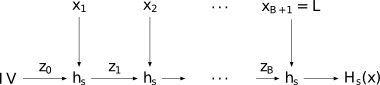
\includegraphics[width=.5\textwidth]{imagens/Merkle-Damgard.png}
  \caption{Diagrama da construção de Merkel Damgrad}
  \label{fig:merkle-damgard}
\end{figure}


\begin{theorem}[Merkle-Damgard]
  Se $\langle Gen, h \rangle$ é resistente a colisão então $\langle Gen, H \rangle$ da forma como definido acima também é resistente a colisão.
\end{theorem}

Construir uma função de hash resistente a colisão para uma mensagem de tamanho arbitrário se resume, portanto, a encontrar uma para mensagem de tamanho fixo que a comprima pela metade.

\subsection{SHA-1}
\label{sec:sha-1}

O {\em Secure Hash Algorithm} (SHA-1) é um algoritmo da família MD4 que recebe uma entrada de tamanho arbitrário $l < 2^{64}$ e produz um {\em digest} de $160$ bits.
Antes de processar a mensagem é inserido um {\em pad} que consiste em uma sequência $10 \dots 0l$ em que $l = |x|$ é o número de bits da mensagem e $|x10 \dots 0l|$ é um múltiplo de 512.
Essa codificação de $x$ é então dividida em blocos $x_0, \dots, x_n$ tais que $|x_i| = 512$.

A função de hash $h$ que alimenta a construção de Merkle-Damgard consiste de 80 rodadas.
Um {\em message schedule} é responsavel por gerar 80 strings $W_0, \dots, W_{79}$ de 32 bits cada a partir do bloco $x_i$ sendo processado. 
Começamos com valores iniciais fixos $A =$ {\tt 67452301}, $B =$ {\tt EFCDAB89}, $C =$ {\tt 98BADCFE}, $D =$ {\tt 10325476}, $E =$ {\tt C3D2E1F0} e alteramos esses valores em cada rodada da seguinte maneira:

\begin{displaymath}
  A, B, C, D, E := (E + f_t(B,C,D) + A_{\lll 5} + W_j + K_t), A, B_{\lll 30}, C, D
\end{displaymath}

A cada 20 rodadas mudamos o valor da constante $K_t$ e da função $f_t$ de forma que o algoritmo precisa definir 4 constantes e quatro funções.
Apenas para matar a curiosidade seguem suas definições:
\begin{enumerate}
\item $K_t :=$ {\tt 5A827999} e $f_t(B,C,D) := (B \land C) \lor (B \land D)$ para $t = 0, \dots, 19$
\item $K_t :=$ {\tt 6ED9EBA1} e $f_t(B,C,D) := B \xor C \xor D$ para $t = 20, \dots, 39$ 
\item $K_t :=$ {\tt 8F1BBCDC} e $f_t(B,C,D) := (B \land C) \lor (B \land D) \lor (C \land D)$ para $t = 40, \dots, 59$
\item $K_t :=$ {\tt CA62C1D6} e $f_t(B,C,D) := B \xor C \xor D$ para $t = 60, \dots, 79$ 
\end{enumerate}

% falar da colisão encontrada no SHA-1 e no MD5

\section{Aplicações}
\label{sec:aplicacoes}

Funções de hash são amplamente utilizadas em protocolos de segurança.
Nesta seção veremos quatro aplicações bastante distintas desses sistemas: um sistema de autenticação bastante popular chamado HMAC, identificação de arquivos e outros tipos de mensagens simples e estruturadas  ({\em fingerprints} e {\em árvore de Merkle}) e derivação de subchaves a partir de outras chaves e a partir de uma senha.

\subsection{HMAC}
\label{sec:hmac}

No capítulo anterior vimos como construir um sistema de autenticação para mensagens de tamanho arbitrário aplicando um esquema similar ao modo CBC.
Alternativamente poderíamos utilizar um hash para produzir um {\em digest} da mensagem de tamanho fixo e então aplicar um sistema de autenticação para mensagens de tamanho fixo no resultado.
Esse sistema é conhecido como {\em Hash-and-MAC}.

Considere um sistema de autenticação $\Pi_M = \langle Gen_M, Mac_M, Ver_M \rangle$ para mensagens de tamanho fixo $l(n)$ e um sistema de hash $\langle Gen_H, H \rangle$ que produz um {\em digest} de tamanho $l(n)$.
O sistema {\em Hash-and-MAC} $\Pi = \langle Gen, Mac, Ver \rangle$ para mensagens de tamanho arbitrário é definido como:
\begin{itemize}
\item $Gen(1^n) := k = \langle k_M, s \rangle$ em que $Gen_M(1^n) := k_M$ e $Gen_H(1^n) := s$
\item $Mac(k, m) := Mac_M(k_M, H_s(m))$
\item $Ver(k, m, t) := \left\{
    \begin{array}{lcl}
      1 & \textrm{se} & Mac(k,m) = t\\
      0 & \textrm{c.c.} &\\
    \end{array}
    \right.$ 
\end{itemize}


\begin{theorem}
  Se $\Pi_M$ é um sistema de autenticação seguro contra falsificação e $\Pi_H$ é um sistema de hash resistente a colisão então a construção $\Pi$ acima é seguro contra falsificação. 
\end{theorem}

\begin{proof}
  Vamos apenas esboçar a prova e deixar os detalhes para o leitor.
  A ideia é a seguinte, suponha que o adversário $\mathcal{A}$ consulte o tag de uma série de mensagens $Q$ e então suponha por absurdo que ele consiga produzir um código válido para uma mensagem $m \notin Q$.
  Neste caso temos duas possibilidades:
  \begin{enumerate}
  \item existe uma mensagem $m' \in Q$ tal que $H_s(m') = H_s(m)$, mas isso contradiz a hipótese que $\Pi_H$ é resistente a colisões
  \item caso contrário $\mathcal{A}$ conseguiu falsificar um código para uma mensagem nova $H_s(m)$ de tamanho $l(n)$ contradizendo a hipótese que $\Pi_M$ é seguro contra falsificação.
  \end{enumerate}
\end{proof}

% Mencionar os protocolos que usam o HMAC

O popular sistema de autenticação HMAC se inspira no esquema apresentado acima usando duas vezes uma função de hash e duas constantes distintas {\tt ipad} e {\tt opad}.
Formalmente definimos o sistema HMAC da seguinte forma:
\begin{itemize}
\item $Gen(1^n) := k \leftarrow \{0,1\}^n$
\item $Mac(k, m) := H_s((k \xor \textrm{\tt opad}) || H_s(k \xor \textrm{\tt ipad})m)$
\item $Ver(k, m, t) := \left\{
    \begin{array}{lcl}
      1 & \textrm{se} & Mac(k,m) = t\\
      0 & \textrm{c.c.} &\\
    \end{array}
    \right.$
\end{itemize}

% argumentar sobre a importância das duas constantes e a relação com o sistema anterior

\subsection{Fingerprints e Árvores de Merkle}
\label{label}

% fingerprint
% árvore de Merkle

\subsection{Funções de Derivação de Chaves}
\label{sec:kdf}

Uma {\em função de derivação de chaves} (KDF) tem como objeto produzir uma chave segura a partir de algum material contendo uma boa quantidade de entropia chamado {\em key material}.
Isso pode ser útil seja porque o {\em key material} não está suficientemente preparado para ser usado como uma chave -- por exemplo no caso de uma senha -- ou quando queremos derivar {\em subchaves} a partir de uma chave inicial.

Formalmente, uma função de derivação de chaves recebe com entrada o {\em key material} $\delta$, o tamanho $l$ da chave a ser produzida e opcionalmente um valor $r$ chamado de {\em salt} e um valor contextual $c$.
Um KDF seguro deve produzir a partir desses valores uma sequência {\em pseudoaleatória} de tamanho $l$.
Tipicamente um KDF consiste de duas etapas: 
\begin{enumerate}
\item {\em extração}: recebe o {\em key material} e opcionalmente uma chave pública ({\em salt}) e produz uma sequência pseudoaleatória de bits de tamanho fixo
\item {\em expansão}: expande o que foi produzido na fase de extração para uma sequência de bits de tamanho $l$.
\end{enumerate}

Uma implementação popular deste modelo é o HKDF que usa apenas o HMAC como primitiva:

\begin{eqnarray*}
  \textrm{PRK}      & := & \textrm{HMAC}(r, \delta)\\
  \textrm{HKDF}(r, \delta, c, l) & := & K(1)||K(2) \dots ||K(t)\\
  K(1)     & := & \textrm{HMAC}(\textrm{PRK}, c||0)\\
  K(i + 1) & := & \textrm{HMAC}(\textrm{PRK}, K(i)||c||i)\\
\end{eqnarray*}

No caso $\delta$ seja uma senha proposta por um usuário, temos um problema a mais, pois tipicamente essas possuem uma entropia baixa e, portanto, estão sujeitas a {\em ataques de dicionário}.
Para mitigar este problema podemos utilizar uma função de derivação de chaves lenta.
Um {\em password based key derivation function} recebe como parâmetro, além do salt $r$, do tamanho $l$ e da senha $\delta$, um valor que estipula o número de ciclos $n$.
Uma implementação popular deste modelo é o PBKDF2:

\begin{eqnarray*}
  \textrm{PBKDF2}(r, \delta, c, n, l) & := & K(1)||K(2)|| \dots ||K(t)\\
  K(i)     & := & U_0^i \xor U_1^i \xor \dots \xor U_n^i\\
  U_0^i    & := & H(\delta||r||i)\\
  U_j^i    & := & H(\delta||U_{j-1}^1)\\
\end{eqnarray*}

Note que a primitiva neste caso é uma função de hash $H$ e que cada $K(i)$ roda $n$ vezes essa função.
O salt impede o preprocessamento de um dicionário e $n$ deve ser grande o suficiente para impedir sua construção {\em a posteriori}.

\section{Exercícios}
\label{sec:exercicios}


\begin{exercicio}
  Mostre que o seguinte sistema não é seguro contra falsificação considerando que o sistema de hash foi construído a partir do paradigma de Merkle-Damgard:
\begin{itemize}
\item $Gen(1^n) := k \leftarrow \{0,1\}^n$
\item $Mac(k,m) := H(km)$
\item $Ver(k,m,t) := \left\{
    \begin{array}{lcl}
      1 & \textrm{se} & Mac(k,m) = t\\
      0 & \textrm{c.c.} &\\
    \end{array}
    \right.$ 
\end{itemize}

\end{exercicio}



\bibliography{ref}
\end{document}